\chapter{引言}\label{chap:introduction}

指令集架构(Instruction Set Architecture, 简称 ISA)的差异导致一个 ISA 上的二进制程序无法在另一个 ISA 上直接运行,这阻碍了 ISA 的创新。
一个新兴的指令集架构因为缺乏软件生态,即使在性能和功耗等指标上存在明显的优势,依旧可能被淘汰,而且即使是主流的 ISA 也必须在严格兼容历史包袱的前提下进行创新。

为了扩展一个 ISA 的生态,架构无关的开源代码可以手动编译,架构有关的开源代码需要专业的工程师维护,这都耗时耗力,而且随着开源软件的更新,需要不断投入人力维护。
而对于闭源程序,例如 PhotoShop 和 Window 操作系统,无法上述的两种方法使其在 Host 上运行。而通过二进制翻译器,可以将客户机( Guest )的二进制代码在( Host )上运行,
为 ISA 的生态建设提供过渡时间。

相比于进程级跨架构二进制翻译器只能翻译应用程序,通过模拟 CPU ,外设,内存和中断,系统级跨架构二进制翻译器可以让客户机操作系统在无需修改源码的情况下在 Host 上运行,
从而消除 ISA 的差异,为指令集架构的创新提供空间。

龙芯公司是国产 CPU 重要力量,其 3A5000 \citep{3A5000/3B5000} 处理器采用 LoongArch \citep{LoongArch} 架构,性能
相比于上一代 MIPS 架构的 3A4000 提升了 50\% \citep{3A5000Release}。作为一个全新的 ISA,LoongArch 和其他 ISA 相同,暂时缺乏丰富的软件生态,因而被限制了应用范围。
然而主流的系统级跨架构二进制翻译器无法满足 LoongArch 的需求。Transmeta Code Morphing 和 IBM 的 daisy 运行需要运行在超长指令字(Very Long Instruction Word, 简称 VLIW 架构指令集上并且含有额外的硬件支持,而主流的高性能 CPU 为乱序多发射的架构,
参考意义较小,QEMU 因为运行在 Host 操作系统上,无法直接访问硬件资源,存在性能瓶颈。而 Captive 和 MagiXen 等二进制翻译器通过硬件加速虚拟化,让二进制翻译器直接访问虚拟机中硬件资源来提升性能,
但是硬件加速辅助虚拟化本身存在开销。

将系统级二进制翻译器直接运行在裸机上,而不是 Host 的操作系统上或者硬件辅助加速虚拟机中,
二进制翻译器可以直接访问所有的硬件资源,绕过 Host 操作系统的抽象,通过 Host 的物理 CPU 直接模拟客户机 CPU,设备直通,硬件 TLB 加速客户机访存等方法
可以尽可能地消除系统级二进制翻译的开销。

本章的组织内容如下,首先简要的介绍二进制翻译的基本原理,分析动态二进制翻译的常用优化技术,分析进程级二进制翻译和系统级二进制翻译器的差别,
并且说明为什么彻底消除指令差异只能通过系统级二进制翻译才能完成,但是系统级二进制翻译也存在劣势,并且从 CPU ,设备,中断和访存四个角度
分别说明。

\section{二进制翻译器概述}

将 Guest 的状态,例如寄存器,保存在内存中,那么一条 Guest 的寄存器之间的赋值指令可以转换为 Host 内存的拷贝操作。
参考 Guest 和 Host 的指令手册,可以知道如何将 Guest 指令翻译为 Host 指令。
在图 \ref{fig:basic_flow} 中,展示了一条 x86 指令翻译为 LoongArch 指令的过程,将 x86 CPU 的状态保存在结构体 GuestCPU 中,
同时一条 x86 指令被翻译为 4 条 LoongArch 指令。

\begin{figure}[!htbp]
	\centering
	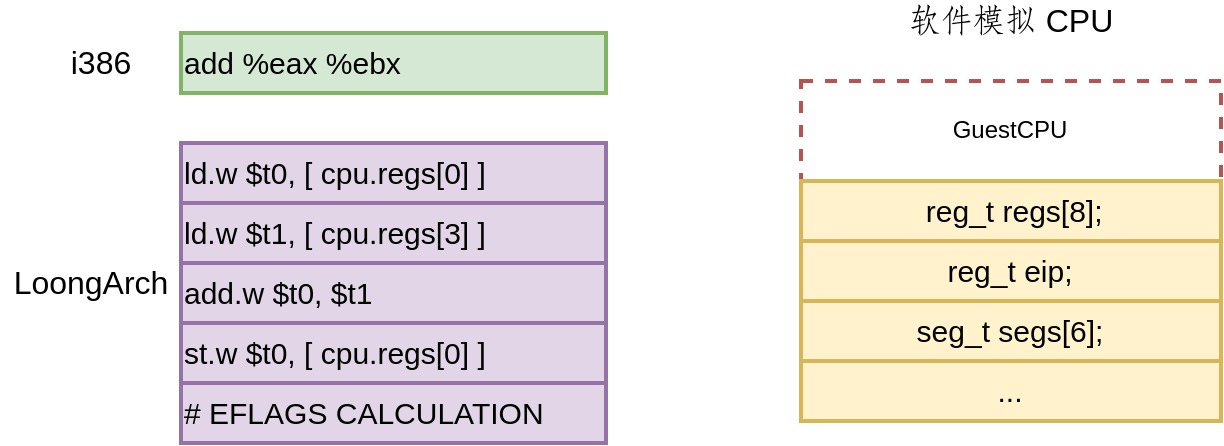
\includegraphics[width=1.0\textwidth]{./images/basic-flow.jpg}
	\caption{从 x86 到 LoongArch 的指令翻译}
	\label{fig:basic_flow}
\end{figure}

\subsection{静态和动态二进制翻译器}
二进制翻译器可以划分为静态二进制翻译器和动态二进制翻译器。
静态二进制翻译器无需客户机程序的运行时信息,可以在 Guest 程序运行之前直接将其翻译为 Host 程序。
而在动态二进制翻译器中,执行和翻译交替进行。

\begin{figure}[!htbp]
	\centering
	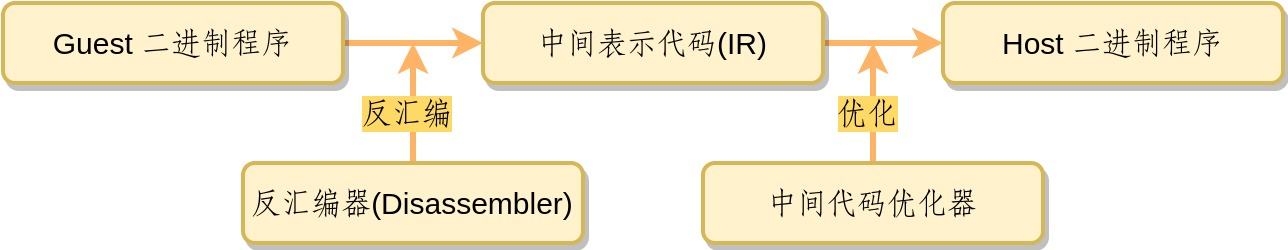
\includegraphics[width=1.0\textwidth]{./images/static-bt.jpg}
	\caption{静态二进制翻译器的执行模型}
	\label{fig:static_bt}
\end{figure}

如图 \ref{fig:static_bt} 所示,静态二进制翻译器首先将 Guest 二进制程序转换为中间代码,
例如 LLVM IR \citep{shen2012llbt},然后进行中间代码优化,最后将中间代码转化为 Host 二进制程序。
因为静态二进制翻译无法获取运行时信息,其使用范围相当有限, 例如:
\begin{itemize}
	\item 通过静态信息,无法正确识别程序的那些部分是数据,那些部分是代码,尤其是在 Guest 二进制程序故意混淆二者的情况下。
	\item 静态二进制翻译无法处理动态生成的代码,例如 just-in-time 编译器。
\end{itemize}

如图\ref{fig:basic_flow2} 所示,在动态二进制翻译中,Guest 代码翻译和代码执行两个行为是交替进行的,并且可以通过运行时信息来指导下一步的翻译行为行为。
\begin{figure}[!htbp]
	\centering
	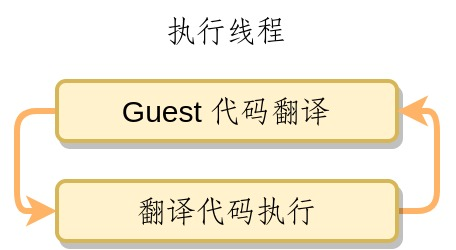
\includegraphics[width=0.4\textwidth]{./images/basic-flow2.jpg}
	\caption{动态二进制翻译器的执行流程}
	\label{fig:basic_flow2}
\end{figure}

为了提升动态二进制翻译器的效率,主流的解决方法一般存在如下的两种基本优化措施:
\begin{enumerate}
	\item 翻译代码缓存
	\item 翻译代码链接
\end{enumerate}

通过\textbf{翻译代码缓存},动态二进制翻译可以避免重复翻译相同的 Guest 代码。
如果一个地址上内存没有被修改过,那么地址上的 Guest 代码翻译出来的 Host 代码可以缓存下来,
当下一次执行到相同位置的时候,可以查询翻译代码缓存(Code Cache)直接获取翻译结果而不是重新翻译。
根据局部性原理,所以只需要少量的内存就可以保证较高的命中率。
如图 \ref{fig:basic_flow3} 是含有 Code Cache 的动态二进制翻译器的执行流程。
\begin{figure}[!htbp]
	\centering
	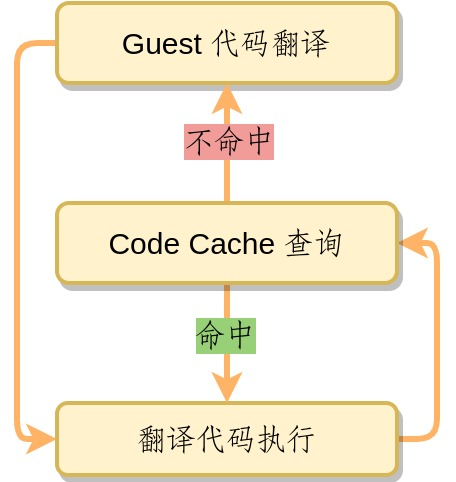
\includegraphics[width=0.4\textwidth]{./images/basic-flow3.jpg}
	\caption{含有 Code Cache 的动态二进制翻译器的执行流程}
	\label{fig:basic_flow3}
\end{figure}
使用 Code Cache 虽然可以减少重新翻译 Guest 代码引入的开销,但是确带来了另一个问题,如果 Code Cache 中对应的 Guest 内存在执行过程中已经发生了修改了,
那么需要将其无效掉,这就是自修改代码(Self Modified Code,SMC) 问题。

通过\textbf{翻译代码缓存},动态二进制翻译可以避免 Guest 和 Host 的上下文切换。
最长的连续的不含有分支指令的指令为一个翻译基本块 (Translation Block, 简称 TB)。因为没有分支指令,可以保证一个 Guest TB 中的指令总是从第一条执行到最后一条,
一个 TB 只会从结束位置跳转到另一个 TB 的开始位置。如果将 Guest 的指令按照 TB 作为最小单位翻译为 Host 指令,那么这些 Host 指令也会组成一个 TB,称之为翻译 TB。
当一个 TB 被执行完成之后,因为如果无法确定下一个 TB 是什么,那么需要在翻译缓存中(Code Cache)进行查询。

进入和退出 Guest 代码执行需要上下文切换,对于进程级的二进制翻译,导致退出的原因包括:
\begin{enumerate}
	\item 系统调用模拟
	\item 信号,例如 Guest 执行触发了段错误,需要将 Host 需要将段错误这个信号转发给 Guest
	\item Code Cache 查询
\end{enumerate}
提升动态二进制翻译器的关键在于,如果尽可能的减少 Guest 的退出,让 CPU 始终在执行 Guest 的翻译代码。

如果不将 TB 链接起来,那么每一个 TB 执行完成之后,都需要进行 Guest 和 Host 的上下文切换以及查询 Code Cache 确定下一个执行的翻译 TB 。
程序中跳转的跳转大多数都是直接跳转,这意味着 TB 的跳转位置往往都是确定的,
,例如 for 结束的位置往往都是会向 for 循环开始的位置跳转,所以每一个 TB 都可以记录下其的跳转目标位置来减少 Code Cache 查询。
其流程图如 \ref{fig:basic_flow4} 所示,TB 1,TB 2,TB 3 被提前执行过一次,被缓存到 Code Cache 中,并且确定 TB 1 跳转到 TB 2,TB 2 跳转到 TB 3,当再次执行的时候,
那么 TB 1 2 3 的执行无需进行 Code Cache 的查询,而 TB 3 到 TB 4 如果无法直接跳转,
那么就通过慢路径进行 Code Cache 查询,如果 Code Cache 中不存在 TB 4,那么就使用二进制翻译引擎重新生成 TB 4。

\begin{figure}[!htbp]
	\centering
	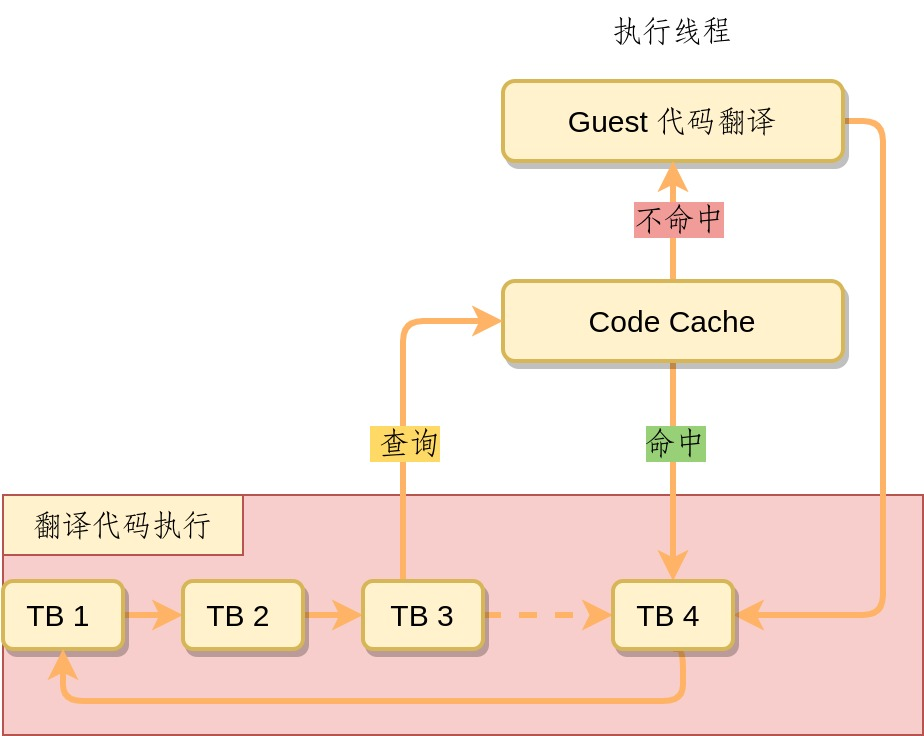
\includegraphics[width=0.8\textwidth]{./images/basic-flow4.jpg}
	\caption{将 Translator Block 链接之后的执行流程}
	\label{fig:basic_flow4}
\end{figure}

如果是直接跳转,其跳转位置可以不依赖运行时信息,TB 的链接之后就无需修改,但是间接跳转取决于运行时信息,其跳转位置会发生改变,TB 链接之后还可能发生修改,如何高效地处理间接跳转也是二进制翻译的难题之一。

\subsection{用户级和系统级二进制翻译器}
根据二进制翻译器所翻译的程序类型,可以将二进制翻译器划分为进程级二进制翻译器和系统级二进制翻译器。

进程级二进制翻译器用于翻译执行 Guest 用户态程序,例如微信和 PhotoShop 等。如图 \ref{fig:user-mode} 所示,Guest 二进制程序不能直接运行到 Host 的操作系统中,需要进程级二进制翻译器来翻译 Guest 指令为 Host 指令,然后执行。

\begin{figure}[!htbp]
	\centering
	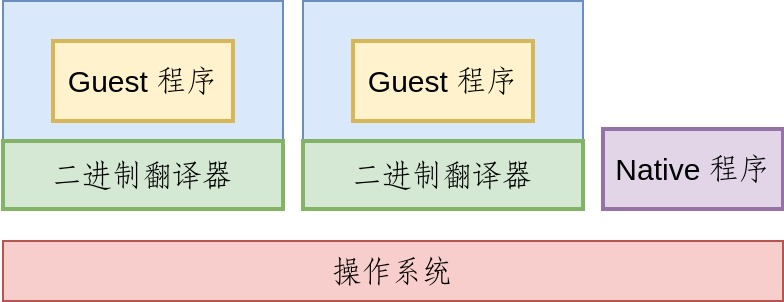
\includegraphics[width=0.7\textwidth]{./images/user-mode.jpg}
	\caption{进程级二进制翻译器}
	\label{fig:user-mode}
\end{figure}

如图 \ref{fig:system-mode} 所示,系统级二进制翻译器则可以翻译执行 Guest 的操作系统,在 Guest 的操作系统上可以运行 Guest 的程序。
\begin{figure}[!htbp]
	\centering
	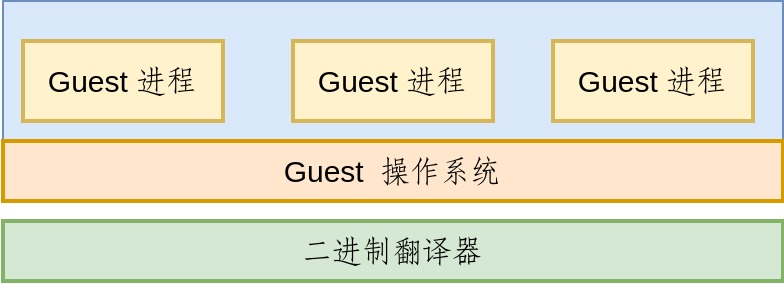
\includegraphics[width=0.7\textwidth]{./images/system-mode.jpg}
	\caption{系统级二进制翻译器}
	\label{fig:system-mode}
\end{figure}

从图 \ref{fig:user-sys-flow} 中可以看出,进程级二进制翻译器和系统级二进制翻译器两者的执行流程类似。
但是,进程级二进制翻译器只需要完成系统调用的模拟,而系统级二进制翻译器需要处理设备,TLB 和的中断。

\begin{figure}[!htbp]
	\centering
	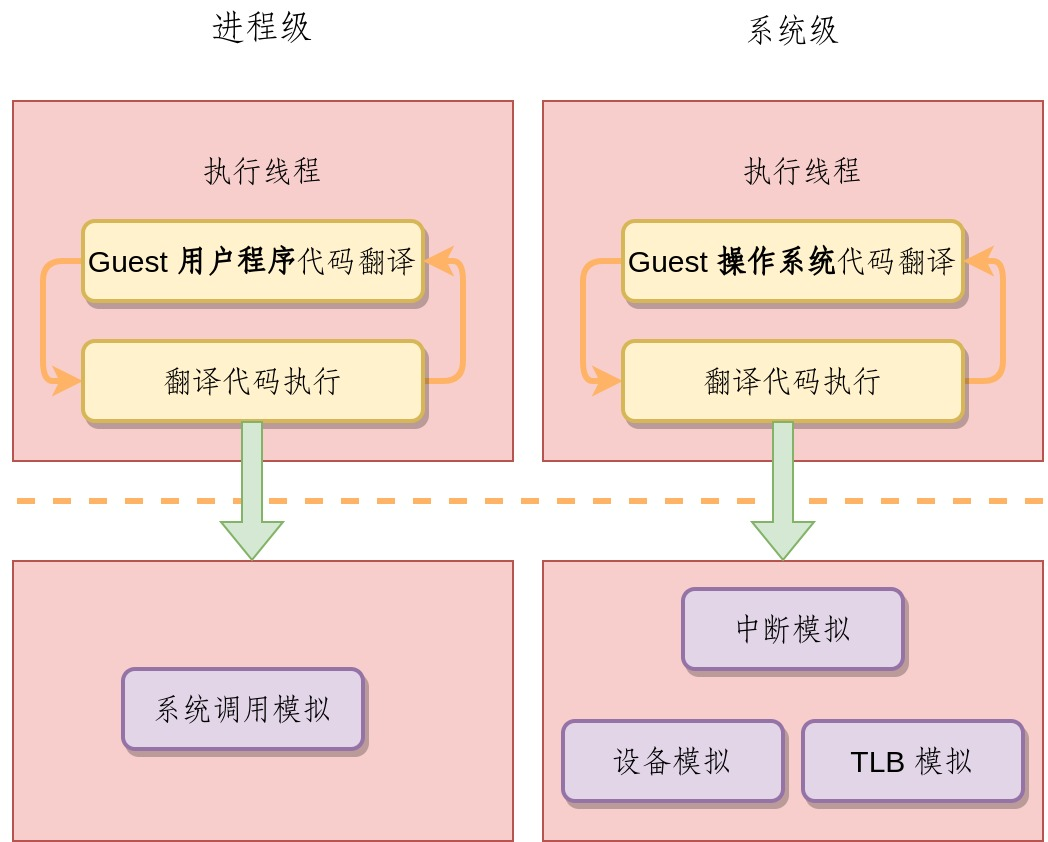
\includegraphics[width=0.7\textwidth]{./images/user-sys-flow.jpg}
	\caption{进程级二进制翻译器和系统级二进制翻译器执行对比}
	\label{fig:user-sys-flow}
\end{figure}

相比于进程级二进制翻译器,系统级二进制翻译器可以做到对于 Guest 用户程序完全透明,例如使用 gdb 调试 Guest 程序,
实际上直接获取到是二进制翻译器的信息,如果 Guest 访问 /proc/\$pid/maps ,如果不经过转换,获取的将会是 Host 的进程地址空间。
更加严重的问题在于,这种不透明可能影响 Guest 程序的运行行为,进而导致 Guest 触发了只有在翻译模式下才会出现的 bug。

Linux 上有丰富的开发工具,但是普通用户需要的日常办公以及娱乐程序却相对缺乏,可以 Linux 操作系统对于支持一个新的指令集持有开放的态度,但是却很难让商业公司微软的 Windows 支持一个新的架构,
为了让 Linux 上可以运行 Windows 程序,
可以采用 Wine \citep{wine} 来进行系统调用的模拟。如果 Guest 程序运行的操作系统和 Host 不相同,例如 Guest 是 Windows 程序,而 Host 是 Linux,那么进程级二进制翻译器需要集成 Wine 来进行系统调用翻译。
而系统级二进制翻译器可以直接运行 Windows 操作系统,然后进一步启动 Windows 程序,消除掉 Wine 引入的性能损失和 bug 。而且 Window 操作系统用户无需切换到操作系统。
但是系统级二进制翻译器因为性能较低,一直难以实用,本课题的意义在于研究如何尽可能的提升系统级二进制翻译器的性能。

\section{系统级二进制翻译的难点}
系统级二进制翻译器和进程级二进制翻译器存在很多共通之处的难点,例如指令翻译,精确异常,自修改代码,间接跳转等。
虽然系统级二进制翻译器相对于进程级二进制翻译器可以保证用户态程序的透明,可以消除系统调用模拟,但是系统级二进制翻译器的性能却低于进程级二进制翻译器的,其原因可以从四个方面说明:

\begin{itemize}
	\item CPU 虚拟化: 虽然进程级二进制翻译器和系统级二进制翻译器的 CPU 模拟的基本过程相同,但是系统级二进制翻译器需要处理系统态指令,例如和硬件辅助虚拟化相关的 vmenter vmexit 等。
	      相同指令,在系统态下的语义也更加的复杂,例如 x86 中的 push / pop 指令,如果是访问 eflags 寄存器,那么其需要被视作一条特权级指令来处理。
	\item 设备虚拟化: 进程级二进制翻译器无需模拟设备,其访问设备都是通过 Host 的系统调用实现的,而系统级二进制翻译器需要提供设备给 Guest 。
	\item 中断虚拟化: 进程级二进制翻译器无需考虑中断,中断的处理是在 Host 的操作系统中进行的。但是系统级二进制翻译器需要模拟 Guest 的中断控制器。
	      Linux 默认的时钟频率是 1000HZ,如果中断不能被高效处理,将会引入显著的开销。
	\item 内存虚拟化: 在进程级二进制翻译器中,Guest 和翻译器访问的空间都是 Host 虚拟地址(Host Virtual Address,简称 HVA),无需进行地址装换。
	      而在系统级二进制翻译器中,Guest 程序的内存访问首先需要进行从客户机虚拟地址(Guest Virtual Address, 简称 GVA)到客户机物理地址(Guest Physical Address,简称 GPA) 的转换,
	      这层的装换如果使用软件模拟,开销会非常大。
	      此外,系统级二进制翻译让 Code Cache 的维护变的更加复杂,在进程级二进制翻译使用 HVA 作为索引查询 Code Cache,
	      而在系统级二进制翻译中,一个进程可以修改从 GVA 到 GPA 的映射,导致相同的 GVA 索引到的翻译 TB 不同,所以查询 Code Cache 则需要使用 GPA,同时 Guest 需要使用 GVA 进行跳转,
	      为了查找其跳转下一个翻译 TB, 系统级二进制翻译在进行 Code Cache 查询之前需要进行一次 GVA 到 GPA 的转换。
\end{itemize}
\section {本文研究内容}
跨架构系统级二进制翻译器是消除指令集差异,扩展指令集壁垒的关键方法,但是却因为翻译性能难以实用。
本文从 CPU 虚拟化,设备虚拟化,中断虚拟化和内存虚拟化四个角度深入分析了跨架构系统级二进制翻译器的挑战,
并且提出了一种全新的系统级二进制翻译器, 裸金属二进制翻译器(Bare Metal Binary Translator,简称 BMBT)来解决这些挑战。

\begin{enumerate}
	\item 在 CPU 虚拟化上,本文验证了使用一个物理 CPU,而不是一个 Host 线程来直接模拟一个 Guest CPU 的可行性。
	      对于裸机上难以调试二进制翻译器的问题,BMBT 采用了用户态,KVM虚拟机和裸机中交叉验证的方法。
	      在 SPEC 2000 定点和浮点测试上,BMBT 分别存在 21\% 和 35\% 的提升。
	\item 在设备虚拟化上,BMBT 设计了裸机上的设备直通, 让 Guest 操作系统直接访问设备,这避免了重新开发 Host 设备驱动,并且消除了设备模拟的开销。
	\item BMBT 提出了让设备中断的模拟和注入在同一个 CPU 上执行的模型,为消除额外的中断标志位检测指令提供了可能。
	      在 fio 的写测试中,BMBT 取得了 189.23\% 的提升。
	\item 利用上 LoongArch 提供的直接映射窗口,BMBT 可以消除所有的 TLB 不命中。同时,BMBT 实现了混合物理页面分配器,可以保证效率和防止物理页面碎片化。
	      memcpy 测试显示 BMBT 有 28.67\% 性能提升。
\end{enumerate}

\section {论文组织结构}
在第一章,首先简单地介绍了二进制翻译,分析静态二进制翻译器无法处理动态生成的代码,以及动态二进制翻译器的两个基本优化技术,然后分析了系统级二进制翻译中的产生性能瓶颈的原因,
最后本文提出裸金属二进制翻译器来克服这些问题。

第二章中,分析三种主流的跨架构二进制翻译器,并且对比了设备虚拟化和内存虚拟化的主要方案。

在第三章中,首先介绍 BMBT 的整体设计思想,然后从 CPU 虚拟化,设备虚拟化,中断虚拟化,内存虚拟化四个角度分析如何实现 BMBT,最后分析 BMBT 的软件结构,说明为何其可以分别在用户态,KVM 虚拟机和裸机上运行。

在第四章中,从 CPU,设备和访存角度分析了 BMBT 的性能 。

第五章中,总结本文的工作,本文已经将基础设施搭建构建完成,未来基于本工作可以进一步优化性能,同时也指出有待完善的地方。

\chapter{相关工作}\label{chap:related_work}
本章首先分析主流的跨架构系统级二进制翻译器,然后分析跨架构系统级二进制翻译器中访存和设备模拟的解决方案。

\section{跨架构系统级二进制翻译器}
全系统模拟可以用于观测体系结构的性能指标,例如 Embra \citep{witchel1996embra} 通过模拟 CPU, MMU (memory management unit,简称 MMU) 和 cache 来计算 cache 的命中率和访存阻塞时间(memory stall time),其通过动态二进制翻译来加速仿真的速度和灵活性。
虽然全系统模拟会使用二进制翻译技术,但是其不会追求性能。

在 Intel 提出了硬件辅助虚拟化 VMX \citep{uhlig2005intel} 之前,VmWare 构建基于二进制翻译的 Hypervisor 来实现虚拟机,例如 VMware 在 x86 平台上可以使用二进制翻译来模拟 x86 Guest 的特权指令。
虽然这种 Hypervisor 实现了系统级二进制翻译,但是其没有跨架构的功能,只能实现从 x86 到 x86 的翻译。

以上两种技术方案虽然都使用了二进制翻译技术,但是其无法同时满足高效和跨架构的要求,能够达到这一要求的主流二进制翻译器主要有如下三种:

\begin{enumerate}
	\item 以 Transmeta Code Morphing 等运行在 VLIW 架构下的二进制翻译器。
	\item 运行在 Host 操作系统上的用户态二进制翻译器,QEMU 。
	\item 以 MagiXen \citep{chapman2007magixen} 和 Captive \citep{spink2016hardware} \citep{spink2020retargetable} 为代表的硬件辅助加速虚拟机中运行的二进制翻译器。
\end{enumerate}

\subsection{VLIW 架构下的二进制翻译器}
基于 VLIW 架构的指令集下存在多个直接运行在系统态中的二进制翻译器,例如 IBM 的 Daisy \citep{ebciouglu1997daisy} ,Transmeta 的 Code Morphing Software \citep{klaiber2000technology} \citep{dehnert2003transmeta} 和 NVidia 的 Denver \citep{boggs2015denver}。
其中以 Transmeta 工作最有代表性。

Crusoe 处理器可以一个时钟周期执行 4 次 VLIW 操作的 CPU ,
其设计目标不是和 x86 架构兼容,而是高性能和低功耗,为此 Crusoe 需要通过 Code Morphing Software 高效地将 x86 指令翻译为 VLIW 指令。

Code Morphing Software 的基本执行流程和图 \ref{fig:basic_flow4} 描绘的基本相同,但是为了提高 Code Morphing Software 的性能,Crusoe 处理提供了一系列的硬件支持:
\begin{enumerate}
	\item 为了实现精确异常,二进制翻译器需要保持翻译指令的顺序和 Guest 指令的顺序一致,这限制了二进制翻译器对于指令调度优化。Crusoe 处理器额外的增加影子寄存器和 gated store buffer 来临时存储一个翻译块的执行结果,
	      只有整个执行块被翻译完成之后,才会提交到寄存器和内存中,
	      而当发生异常之后,会回滚到翻译块的开始位置并且按照 Guest 指令顺序重新翻译执行。
	\item 因为翻译器无法区分访存的目标是物理内存还是 Memory-mapped I/O(简称 MMIO),因此访存不能乱序执行。Crusoe 提供了一个在 Memory-mapped I/O 中乱序执行触发异常的硬件机制,从而保证可以在物理内存上乱序执行,在 Memory-mapped I/O 上顺序执行。
	\item 对于 SMC ,如果 Guest 写了含有代码的物理页面,需要将该物理页面上关联的所有翻译代码全部无效掉,但是如果该页面同时存在代码和数据,而客户机在写数据,那么就没有必要无效掉该页关联的翻译代码。
	      Crusoe 提供更加小粒度的翻译代码保护来区分代码和数据,从而避免不必要的翻译代码无效,降低自修改代码带来的性能开销。
\end{enumerate}

Code Morphing Software 可以高效地实现系统级跨架构二进制翻译,但是其性能提升主要得益于额外的硬件辅助机制。同时基于 VLIW 的软件生态系统难以建立,
无法达成最终构建基于该 ISA 的生态系统的目标。现代的主流 CPU 设计是乱序多发射的架构,在软件上和 VLIW 存在较大差别,VLIW 的二进制翻译器的代码难以直接复用。

\subsection{QEMU}
QEMU \citep{bellard2005qemu} 是虚拟化解决方案的集大成者,其可以运行在多种操作系统上,包括 FreeBSD,Linux, MacOS 和 Windows,并且支持多种虚拟化技术,例如 KVM 和 HyperV。
QEMU 同时支持虚拟机镜像,热迁移等功能。

在二进制翻译方面,QEMU 同时支持进程级二进制翻译和系统级二进制翻译。在设备虚拟化方面,QEMU 支持 PCIe 设备直通,设备模拟和 virtio 协议。
相比于 Transmeta 等二进制翻译器只能实现一种 Guest 指令集到另一种 Host 指令集的翻译,QEMU 可以支持 Alpha, ARM, x86, MIPS 等 20 种指令集之间的互相翻译。
在同一个指令集下, QEMU 还可以模拟各种 CPU 的型号和主板型号,而且可以根据主板配置自动生成高级配置和电源管理接口 (Advanced Configuration and Power Management Interface,简称 ACPI 表提供给 Guest。

QEMU 作为一个优秀的开源项目,其代码运行稳定,并且在一些关键问题上提供了解决方案:
\begin{enumerate}
	\item 提供了间接跳转,自修改代码,精确异常,中断等二进制翻译难点的基本解决方案。
	\item 较好的模拟了 x86 上的各种特有的设备,例如其中断控制器 IOAPIC, Local APIC 和 PIC。
	\item 模拟特权级指令,例如 CPUID 指令。
	\item FPU 以及 SIMD 指令的模拟。
\end{enumerate}

但是,QEMU 的兼容性和可扩展性降低了其作为一个系统级跨架构二进制翻译的性能。
\begin{enumerate}
	\item QEMU 为了同时兼容多种技术,例如 KVM,不能将其运行在系统态,运行在用户态让系统级二进制翻译无法直接访问硬件资源,这正是本文的想要解决的问题。
	\item 为了支持多个指令集之间的二进制翻译,QEMU 使用 Tiny Code Generator(简称 TCG)来作为中间代码。
	      一个新的指令集如果想要被 QEMU 支持,只需要实现该指令集到 TCG 的翻译和 TCG 到该指令集的翻译。
	      虽然中增强了代码复用,降低了开发难度,但是导致了翻译效率的下降。
	      例如,为了将 x86 翻译为 LoongArch,QEMU 会首先将 x86 指令翻译为 TCG, 然后将 TCG 翻译为 LoongArch 指令。
	      在简化模型的情况下,如果一条 x86 翻译为 2 \textasciitilde 3 条 TCG 指令,
	      一条 TCG 指令翻译为 2 \textasciitilde 3 LoongArch 指令集,
	      那么一条 x86 指令将会膨胀为 4 \textasciitilde 9 LoongArch 指令,在 LoongArch CPU 上使用二进制翻译器执行 x86 程序的性能就很难超过 25\% 了。
	      此外,TCG 作为一个中间表示代码,QEMU 对于其进行的中间代码优化相当有限。
	\item 为了模拟多种网卡,存储,CPU,主板和总线等,QEMU 构建了大量的抽象层次,例如 QEMU Object Model 等,就系统级二进制翻译而言,这些设计增加了维护难度,降低了软件性能。
	\item 为了支持多个架构,QEMU 在尽量采用各个架构的通用属性来,而没有使用上一些 ISA 的特性,例如 LoongArch 中的二进制翻译扩展。
\end{enumerate}

BMBT 无需支持各种硬件辅助虚拟化技术,因此可以直接运行在裸机上,从而简化软件层次,

\subsection{硬件辅助虚拟化加速二进制翻译}
MagiXen 在 Xen \citep{barham2003xen} 的基础上构建一个特殊的 DomU,MagiDomain,如图 \ref{fig:MagiXen} 所示,
其中 IA-32 EL \citep{1253195} 是 Intel 开发的闭源进程级二进制翻译器,为了支持系统级二进制翻译,当 IA-32 EL 的执行过程中遇到了特权指令,Hypercall 指令,硬件中断和异常的时候,
需要退出到 MagiXen 装换层来处理。当处理完成之后,会恢复 IA-32 EL 的状态,继续执行。

因为 QEMU 的性能低于 IA-32 EL,所以 MagiXen 采用了后者,但是 IA-32 EL 是闭源商业软件,导致 MagiXen 无法进一步修改二进制翻译器,因而存在诸多限制:
\begin{enumerate}
	\item 可能因为商业原因被 Intel 限制。
	\item IA-32 EL 的编程接口不清晰,基于 IA-32 EL 开发非常困难。
	\item x86 不是可虚拟化架构,而 IA-32 EL 作为进程级二进制翻译器,对于敏感指令不会产生 trap,所以必须修改 Guest OS 将其中的特权指令进行替换。
\end{enumerate}

\begin{figure}[!htbp]
	\centering
	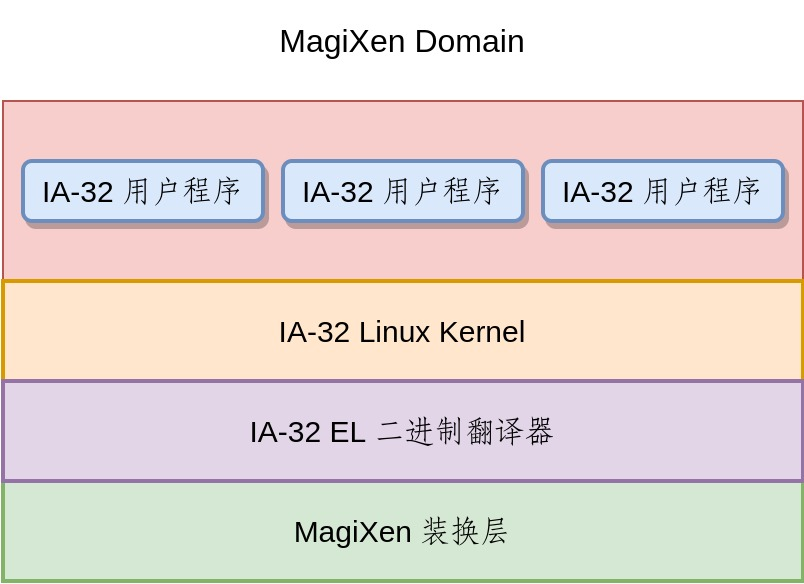
\includegraphics[width=0.6\textwidth]{./images/MagiXen.jpg}
	\caption{MagiXen 软件架构}
	\label{fig:MagiXen}
\end{figure}

因为 Guest OS 是半虚拟化的操作系统,其设备虚拟化和中断虚拟化的处理相对于全虚拟化要简单高效。
而访存虚拟化,MagiXen 运行在系统态中,所以其可以直接访问硬件 TLB ,
在其中存储 Guest x86 的虚实地址空间的映射,当发生 TLB 不命中的情况,让 Xen 直接填充 Guest x86 的页表。

同样是利用硬件辅助虚拟化技术,Captive 则是利用 KVM 创建了一个裸机环境,在其中构建从 ARM 的 x86 的系统级二进制翻译器。

如图 \ref{fig:captive} 所示,Captive 大致分为三个部分:
\begin{enumerate}
	\item 二进制翻译 Hypervisor,其主要和 Linux kernel 的 KVM 模块交互,从而创建 x86 虚拟机。
	\item X86 unikernel,其运行在 x86 虚拟机中,为二进制翻译器提供一个执行环境。
	\item 二进制翻译器,通过体系结构描述语言生成。
\end{enumerate}

\begin{figure}[!htbp]
	\centering
	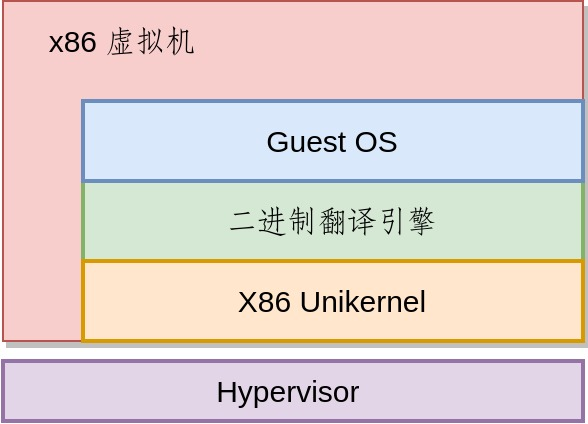
\includegraphics[width=0.5\textwidth]{./images/captive.jpg}
	\caption{Captive 软件架构}
	\label{fig:captive}
\end{figure}

在 CPU 虚拟化上,QEMU 的指令翻译引擎是手动构建的,Captive 是首先通过架构描述语言构建出来静态单赋值(Static Single Assignment, SSA)形式的中间代码,
经过优化之后会生成二进制翻译函数构成的指令翻译引擎。
执行引擎首先解码,然后对于每一个解码的指令调用指令翻译函数,翻译函数会生成中间代码,在其中会进行数据流和控制流分析,最后生成目标代码,也就是 x86 代码。

通过硬件辅助虚拟化,Captive 可以利用上硬件 TLB 从而加速访存,但是也带来问题:
\begin{enumerate}
	\item 为了能够尽量的减少 vmexit 带来的性能开销,Captive 需要重新构建了一个新的 Hypervisor ,而不是利用现有的 Hypervisor,例如 QEMU 或者 kvmtool \citep{kvmtool}。
	\item 因为 Hypervisor 运行在 Linux 的用户态,并且需要频繁和 KVM 模块交互,其还是无法消除掉 Linux 软件栈和系统调用的开销。
\end{enumerate}

\section{跨架构二进制翻译器关键技术}

\subsection{设备虚拟化}
设备虚拟化主要存在三种解决方案

第一种方法是\textbf{设备模拟}。
QEMU 模拟的设备种类齐全,架构清晰,本文以 QEMU 作为例子分析设备模拟的基本运行过程。
在 Guest 中网络应用程序 curl 发送一个网络包,如图 \ref{fig:kernel_stack} 所示,其会调用一个调用系统调用进入到 Guest 的内核,经过 Guest 内核的网络栈,
每经过一层协议,网络包就会增加一个协议头,最后使用网卡,例如 e1000e 网卡,将封装完全的网络包发送出去。

CPU 向 e1000e 的 MMIO 空间中写入命令来控制 e1000e 网卡发送网络包。现代操作系统中,CPU 不是直接使用物理地址问设备,
例如 Linux 中的 ioremap 机制,而是使用虚拟地址来访问设备,虚拟地址和物理地址的装换通过 MMU 完成。
如图 \ref{fig:qemu_device_user} 所示,Guest CPU 写 e1000e 网卡的 MMIO 空间行为可以被 QEMU 硬件内存管理模拟机制(简称 softmmu)捕获下来,通过设备访问分发,QEMU 可以知道被访问的设备是 e1000e 网卡,
之后调用 e1000e 模块注册的钩子函数,将网络包根据网络协议逐层拆开,最后调用 Host 的系统调用将数据发送取出,进入到 Host 内核之后的流程和 \ref{fig:kernel_stack} 相同。

\begin{figure}[!htbp]
	\centering
	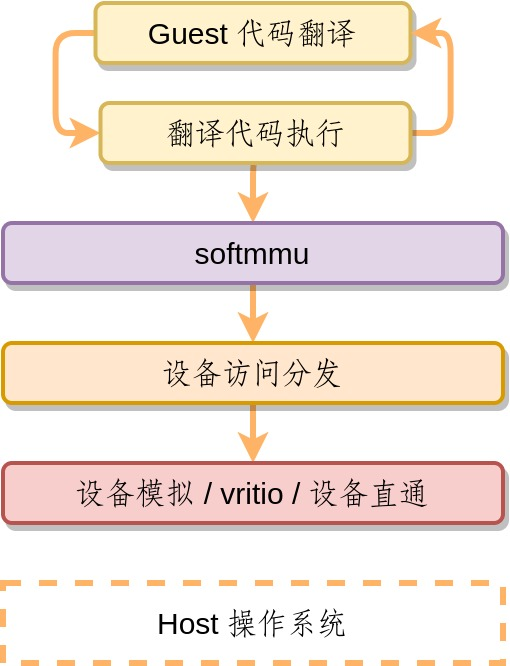
\includegraphics[width=0.6\textwidth]{./images/device-virtualization.jpg}
	\caption{运行在用户态中系统级二进制翻译器设备模拟过程}
	\label{fig:qemu_device_user}
\end{figure}

\begin{figure}[!htbp]
	\centering
	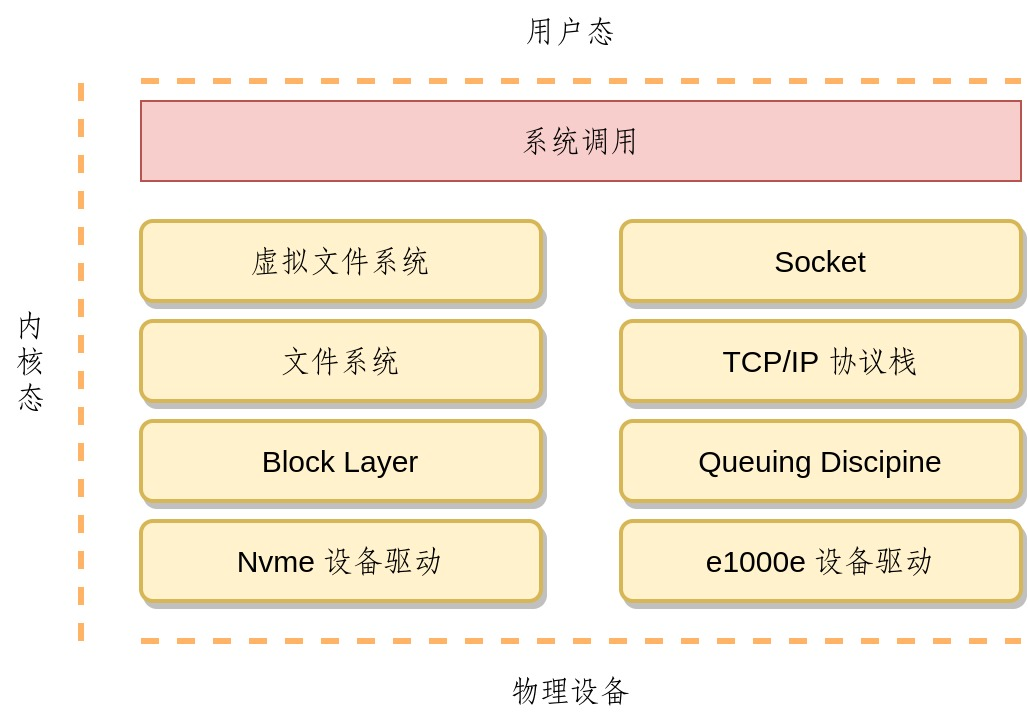
\includegraphics[width=0.8\textwidth]{./images/linux-stack.jpg}
	\caption{Linux 内核的网络栈和存储栈}
	\label{fig:kernel_stack}
\end{figure}

设备模拟存在两个导致其性能下降的问题:
\begin{enumerate}
	\item 访问到 Host 的物理设备需要同时经过 Guest 和 Host 的网络栈
	\item Hypervisor 需要精确的模拟复杂的物理设备接口。
\end{enumerate}

第二种设备模拟方法是 \textbf{半虚拟化}。
为了完整地模拟设备,例如 e1000e 网卡,Hypervisor 需要构建一个复杂的前端来精确地模拟物理网卡,虽然 QEMU 可以让模拟行为执行在 IO 线程中,但是复杂的设备模拟还是会降低设备延迟和吞吐量。
半虚拟化的代表是 virtio \citep{russell2008virtio},其被 Windows,Linux 等操作系统和 QEMU,firecracker 等 Hypervisor 支持。
virtio 协议让 Hypervisor 不再去模拟具体的物理设备,Guest 操作系统和 Hypervisor 按照 virtio 协议的标准来交互。
对于运行在 Linux 上的 QEMU,为了支持 virtio,Linux 需要实现 virtio 前端驱动,QEMU 需要实现 virito 后端驱动,两者通过 virtio 协议沟通。

virtio 协议的设计目的就是提高性能,其让 Hypervisor 无需精准的模拟复杂的物理设备的接口,但是 virito 也无法避免数据需要同时经过 Host 和 Guest 的软件栈才能到达 Host 物理设备的问题。
此外,virito 要求 Guest 操作系统含有对应的 virito 设备驱动,限制了其使用范围。

第三种是 \textbf{设备直通}。 设备模拟和半虚拟化不同,设备直通可以让 Guest 直接操作物理设备。

在 Linux 操作系统,可以通过 VFIO \citep{williamson2012vfio} 来实现设备直通。
如图 \ref{fig:vfio} 所示,Linux kernel 中的 VFIO 利用 IOMMU 可以安全地实现 PCIe 设备直通,从而可以让 Guest 设备驱动直接访问到 PCIe 设备,
而设备中断则是由 Host Linux 接收管理,通过 eventfd 方式通知 QEMU,最后经过模拟的 Guest 中断控制器注入到 Guest 中。

\begin{figure}[!htbp]
	\centering
	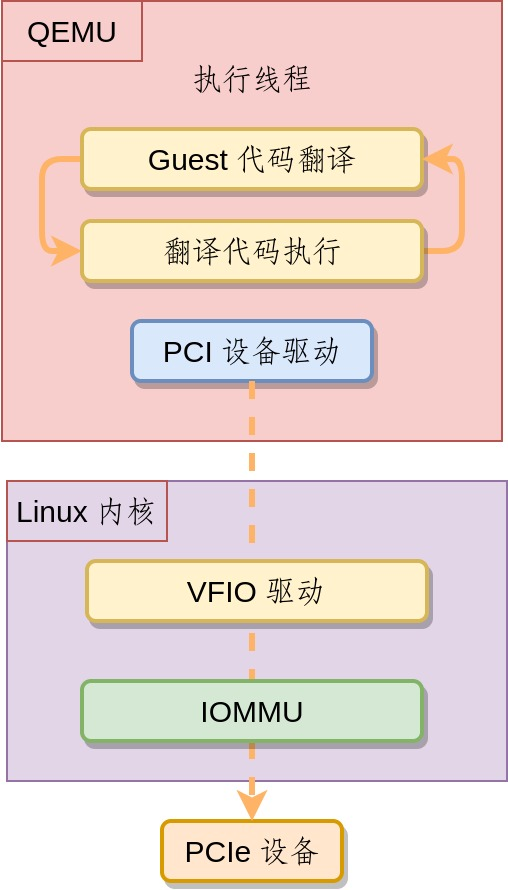
\includegraphics[width=0.4\textwidth]{./images/vfio.jpg}
	\caption{VFIO 设备直通}
	\label{fig:vfio}
\end{figure}

虽然 VFIO 设备直通让 Guest 访问设备几乎没有性能损失,但是存在如下限制:
\begin{enumerate}
	\item 能够直通的设备仅仅限于 PCIe 设备,大多数主板上包含的串口,hpet 等非 PCIe 设备无法直通。
	\item 如果 PCIe 设备不支持 Virtual Function,那么该设备需要被独占。而设备模拟和 virtio 可以实现设备复用。
\end{enumerate}

BMBT 的设备虚拟化方法也采用的是设备虚拟化的方式,但是除了 PCIe 可以直通,还是支持串口等设备的直通。

\subsection{内存虚拟化}\label{subsection:memory_virt}
访存是系统级二进制翻译性能低于进程级二进制翻译器的关键原因。如图 \ref{fig:user-as} 所示是 Linux 的进程地址空间。
操作系统负责维护页表,页表中存储了将进程地址空间的虚拟地址映射到物理页面的信息。例如 x86 支持 32bit 虚拟地址空间,一个虚拟地址划分为 10bit 10bit 12bit,进程的 cr3 寄存器保存根页表地址,
如果 TLB 不命中,那么需要遍历页表,首先使用高 10bit 作为偏移来访问根页表来确定次级页表地址,然后使用中间的 10bit 作为偏移访问次级页表获取目标物理页面的地址,最后进行一次访存读写数据,
原本一次访存被放大为 3 次。 LoongArch 的虚拟地址空间为 $2^{64}$ 的大小,可以配置 48bit 来索引页表,如果 LoongArch 的页大小为 16k,那么 48bit 可以划分为 11bit 11bit 11bit 11bit 14bit ,
类似的,如果 TLB 不命中,将会一次访存会被放到为 5 次访存。

\begin{figure}[!htbp]
	\centering
	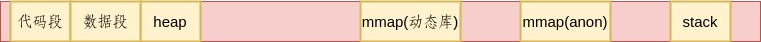
\includegraphics[width=1.0\textwidth]{./images/user-as.jpg}
	\caption{Linux 进程地址空间}
	\label{fig:user-as}
\end{figure}

在进程级二进制翻译中,如图 \ref{fig:user-as2} 所示,将二进制翻译器占用的虚拟地址空间约束到指定的区间中,
可以通过截获 mmap 等访问进程地址空间相关的系统调用,隐藏这些被占用的区间,
让 Guest 以为完全占有 Host 操作系统提供的进程地址空间,此时 GVA 等于 HVA,其访存操作无需使用 softmmu 进行虚拟地址到物理地址的转换,而是和 Host 的普通用户进程相同,
使用 Host 的 TLB 来加速访存,因此和访存相关的指令在进程级二进制翻译器中其性能损失和其他指令无明显差别。

\begin{figure}[!htbp]
	\centering
	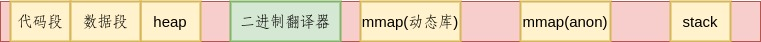
\includegraphics[width=1.0\textwidth]{./images/user-as2.jpg}
	\caption{进程级二进制翻译器的地址空间}
	\label{fig:user-as2}
\end{figure}

但是进程级二进制翻译提供给 Guest 的虚拟地址空间难以做到透明。在 LoongArch 平台上,页大小为 16K ,而运行的 x86 程序认为自己运行在页大小为 4k 的硬件上。如果 Guest 连续映射 4 个页面,分别设置
不同的四个属性,例如为可读,可读可写,可写,可执行,那么 Host 只能设置上所有的属性,也就是可读可写可执行。这种设置冗余权限的方法会引入
冗余的问题。如图 \ref{fig:16k} 展示了一个更加严重的问题,如果进程 A 首先映射一个 4K 页面,因为 Host 是 16K ,实际上会自动将
剩余的 3 个 4K 页面映射,然后 A 将此页面共享 B 进程中,但是如果 A 进程想要将第二个页面和 C 进程共享,这个操作是无法完成的。

\begin{figure}[!htbp]
	\centering
	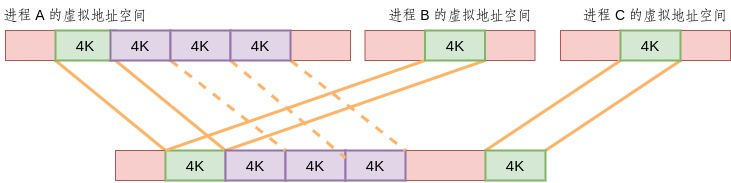
\includegraphics[width=1.0\textwidth]{./images/16k.jpg}
	\caption{进程级二进制翻译器的页共享}
	\label{fig:16k}
\end{figure}

系统级二进制翻译可以给 Guest 提供一个完全透明的进程地址空间,这是因为提供的 Host 虚拟地址空间是用于模拟 Guest 物理内存而不是 Guest 虚拟地址空间。
如图 \ref{fig:sys-as2} 所示,如果系统级二进制翻译中运行在 Linux 操作系统上,其可以使用 mmap 来申请一块连续的虚拟地址空间来模拟物理内存。

\begin{figure}[!htbp]
	\centering
	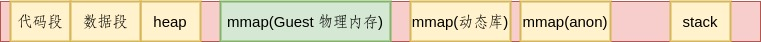
\includegraphics[width=1.0\textwidth]{./images/sys-as2.jpg}
	\caption{系统级二进制翻译器的地址空间}
	\label{fig:sys-as2}
\end{figure}

图 \ref{fig:sys-as} 展示了 QEMU 中 GVA 到 GPA 的映射过程,Guest 访问物理内存,首先根据 Guest 的页表进行从 GVA 到 GPA 的装换,然后根据 mmap 的偏移量计算 GPA 的装换 HVA,
最后根据 Host 的页表实现从 HVA 到 HPA 之间的装换。可以使用软件 TLB 加速 Guest 的访存速度,在软件 TLB 中存储 GVA 到 HVA 的映射,
在二进制翻译器生成访存指令的时候,可以首先生成软件 TLB 访问的指令,如果命中,那么使用 HVA 直接访问。
如果软件 TLB 不命中,Guest 需要进行 3 次访存,如果 Host 的 TLB 的访问也不命中,那么每次 Guest 的访存会被放大 5 倍,也就是一共 15 次访存。

\begin{figure}[!htbp]
	\centering
	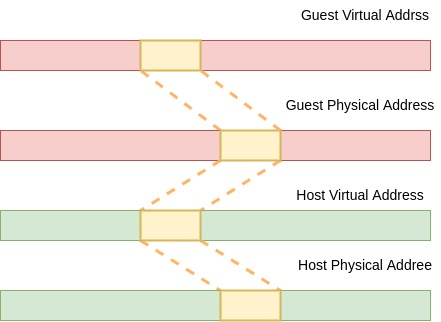
\includegraphics[width=0.7\textwidth]{./images/sys-as.jpg}
	\caption{QEMU 中 GVA 到 GPA 的映射过程}
	\label{fig:sys-as}
\end{figure}

如图 \ref{fig:softmmu} 所示,在中 QEMU ,一条 x86 访存指令翻译一共会被翻译为 14 条 LoongArch 指令。首先
将根据 GVA 索引到一项 CPUTLBEntry,然后对比 TLB tag 是否相等,如果相等,使用 CPUTLBEntry 中存储的 HVA 来访问。
即使 TLB 全部命中,除了三条 GVA 加载指令,一条 x86 Guest 访存指令也额外的会生成 11 条 TLB 模拟指令。
图中演示的 x86 指令只有一个操作数需要访存,如果存在多个,每一个访存都会引入额外的 11 条 TLB 模拟指令。
因为 TLB 模拟,一条 Guest 访存指令会膨胀为多条 Host 指令,同时访存指令在程序中出现的频率很高,
导致系统级二进制翻译器的性能远远低于进程级二进制翻译器。

\begin{figure}[!htbp]
	\centering
	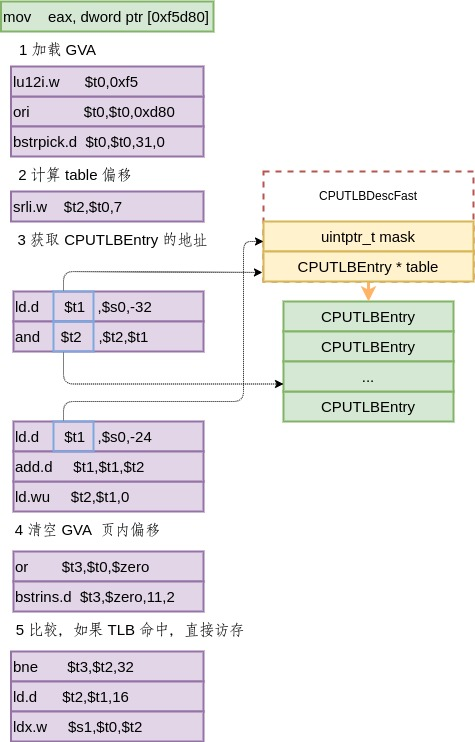
\includegraphics[width=0.7\textwidth]{./images/softmmu.jpg}
	\caption{一条 x86 访存指令的翻译过程}
	\label{fig:softmmu}
\end{figure}

可以使用 Host 的硬件 TLB 来加速 Guest 访存,其大致方案如下:
\begin{enumerate}
	\item 将 Host 的虚拟地址空间中 0 到 4G 预留给 Guest 。
	\item 建立对于 0 \textasciitilde 4G 的 TLB 填充函数。 在 TLB 填充函数的行为中,使用软件遍历 Guest 的页表,
	      如果 Guest 页表中含有 GVA 到 GPA 的映射,将其填充到 Host 硬件 TLB 中,并且返回到触发 TLB 异常的指令重新执行
	      否则在 Guest 中触发 page fault 异常。
\end{enumerate}
使用硬件 TLB 加速之后,如图 \ref{fig:hamt} 所示, 除了加载 GVA 指令之外,可以实现一条 LoongArch 指令来模拟一条 Guest 的访存指令。
如果访存命中,因为 0 \textasciitilde 4G 范围的硬件 TLB 存放的是 Guest 的 GVA 到 HPA 的映射,所以可以硬件 TLB 中完成翻译并且访存,
如果不命中,进入到 TLB 充填函数中。

\begin{figure}[!htbp]
	\centering
	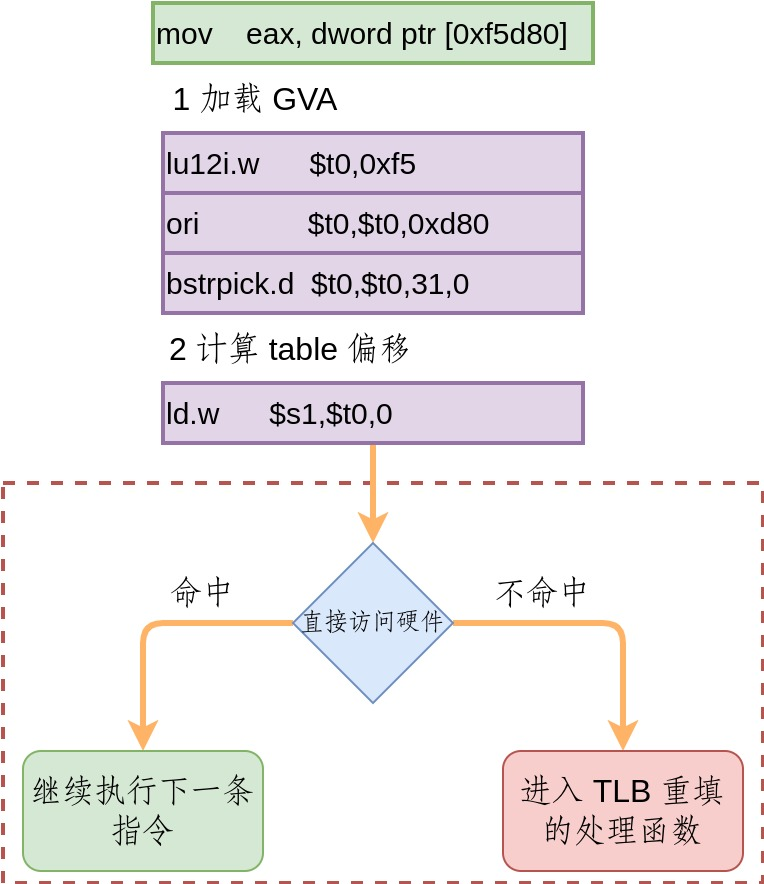
\includegraphics[width=0.7\textwidth]{./images/hamt.jpg}
	\caption{硬件 TLB 辅助 Guest 访存指令翻译过程}
	\label{fig:hamt}
\end{figure}

如果二进制翻译器直接运行在用户态,无法直接访问 Host 的硬件 TLB ,而是需要使用系统调用操控内核模块来实现。
每次硬件 TLB 不命中的时候,都需要进行一次系统调用,其中系统态和用户态的切换开销就会超过硬件 TLB 加速的收益。
为了能够直接访问硬件 TLB,必须直接进入到系统态中运行二进制翻译器。

进入系统态的方法有三种,第一种是在虚拟机中执行,第二种是在 Dune 中执行,
第三种是直接在硬件上执行。前两种方式是进入到 non-root 模式下的 Guest 态,而第三种方式进入到 root 模式下的 Guest 态。
无论是虚拟机中还是 Dune 中,都需要额外的硬件支持,并且引入开销。

\textbf{虚拟机中执行}。
如果二进制翻译器运行在硬件辅助加速的虚拟机中的系统态中,例如 MagiXen ,Captive 和 HyperMAMBO-X64 \citep{d2017hypermambo} 。
因为 QEMU 同时支持构建虚拟机和二进制翻译,所以可以让 QEMU 作为二进制翻译器运行在 QEMU 构建的虚拟机中。

\textbf{在 Dune 中执行} \citep{belay2012dune}。通过 Dune 可以构建一个进程级虚拟机,将运行在用户态的二进制翻译器,例如 QEMU,执行在 Guest 的系统态从而直接
访问硬件 TLB \citep{faravelon2018acceleration}。Dune 需要构建一个内核模块,随着内核的更新,Dune 也必须更新其实用的内核编程接口,而且 Dune 的内核模块的稳定性较差。Dune 对于多线程的支持也相当有限。
Loongson-Dune \citep{loongsonDune} 使用 Linux 的 KVM 模块来替代 Dune 的内核模块来解决这些挑战。在下文中,Dune 指的是 Loongson-Dune 。

运行在 Dune 中的程序,例如 QEMU,首先被 Host 操作系统正常的加载,然后 QEMU 调用 Dune 的函数,在其中 Dune 利用 QEMU 的运行时信息,例如寄存器的内容初始化虚拟机的环境,来初始化虚拟机的状态,
然后进入启动虚拟机。在虚拟机中,只需要保证 GVA 等于 HVA,那么 Host 内存中的改动,在 Guest 中可以在相同位置观测到,反之也是如此。Guest 的系统调用,在 Host 中使用相同参数调用,
从内存修改的角度,等价于 Guest 直接调用该系统调用。

如图 \ref{fig:dune} 所示,一个用户态进程不能直接执行特权级指令,而是需要通过系统调用来请求内核来执行,当一个进程运行在 Dune 中,如果进行系统调用,会触发如下 6 个步骤:
\begin{enumerate}
	\item 将会跳转到 Dune 预先设置的位置,将参数保存到约定的地址上,然后执行 hypercall 指令,从 Guest 态中退出到 Host 的系统态中,也就是 kvm 中。
	\item kvm 检测到这是一个特殊的 hypercall 指令,会退出到用户态,进入到 Dune 的执行代码中,从 Dune 的视角是 ioctl 返回。
	\item Dune 解析在步骤 1 中保存的系统调用参数,并且使用这些参数调用系统调用,在这个步骤中,Dune 完成了 Guest 的系统调用在 Host 代理。
	\item 系统调用返回之后,Dune 会将返回值保存到和 Guest 约定的地址中。
	\item Dune 调用 ioctl 进入到 kvm 中。
	\item 从 kvm 进入到 Guest 中,执行 hypercall 指令的下一条指令,然后恢复上下文环境,跳转到 Guest 执行系统调用的下一条指令。
\end{enumerate}

\begin{figure}[!htbp]
	\centering
	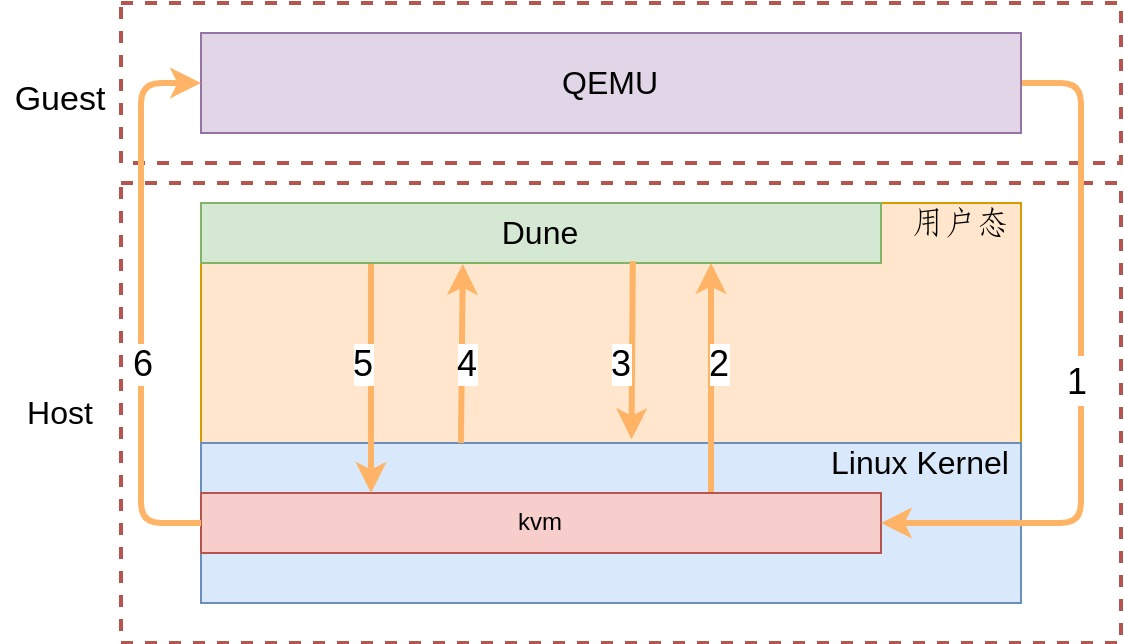
\includegraphics[width=1.0\textwidth]{./images/dune.jpg}
	\caption{Loongson Dune 的运行过程}
	\label{fig:dune}
\end{figure}

相对于方法一,利用 Dune 无需构建一个 unikernel,这减少了工程量,增加了项目的稳定性和可维护性,但是使用 Dune 方案也存在局限性:
\begin{enumerate}
	\item Dune 无法提供一个完全透明的运行环境。例如,用户进程原本 segment fault 的行为会被 KVM 理解为虚拟机运行异常,
	      这会和其他的错误以相同的错误码提供给 Dune, Dune 无法区分。
	      此外,信号处理函数还是会运行在 Host 态中。
	\item 在 Dune 中运行的程序的系统调用会导致 Guest Host 的上下文切换,以及系统态和用户态的切换。虽然可以通过修改内核的方法,
	      合并上述步骤中的 2 3 4 5 步骤为在内核中直接调用系统调用的处理函数,但是还是无法消除 Guest 和 Host 的切换。
	\item Dune 的运行基础是系统调用截获,如果 Guest 执行系统调用指令,例如 x86 的 int 0x80 ,然后跳转到特定的位置,在该位置让 Guest 从虚拟机中退出,进而模拟系统调用。
	      但是 Linux 中 vdso 机制可以将内核中的只读数据直接提供给用户进程,也就是说执行该系统调用无需执行 int 0x80 指令,也不会跳转到特定的位置,那么该系统调用无法被截获。
\end{enumerate}

第三种方法是直接 \textbf{在裸机上中执行}。BMBT 采用的是这种方法,此方法可以避免硬件辅助虚拟化带来的开销。

\section{小结}
本章首先分析主流的跨架构系统级二进制翻译器,基于 VLIW 架构的 Transmeta Code Morphing 等系统态二进制翻译器虽然可以
实现较高的二进制翻译器效率,但是其是在特殊的硬件条件下实现的。QEMU 作为广泛的应用的虚拟化方案,因为运行在 Host 的操作系统上,
无法直接访问硬件资源,并且存在较深的软件栈,性能不高。而运行在硬件辅助加速虚拟机中的二进制翻译器虽然可以直接访问系统资源,
但是却引入了虚拟机的开销。此外本小结分析了实现系统级二进制翻译的两个关键问题,内存虚拟化和设备虚拟化。
只有利用上硬件 TLB 加速才可以高效实现内存虚拟化,可以硬件辅助加速虚拟机,Dune 或者直接在裸机上运行这三种方法实现硬件 TLB 的访问。
可以通过设备模拟,半虚拟化以及设备直通来实现设备虚拟化,

\chapter{BMBT 的设计和实现}\label{chap:bmbt}

\section{BMBT 总体设计思路}
BMBT 的设计目的是尽可能提高跨架构二进制翻译器的性能,因此无需在不必要的功能上浪费性能。全系统态模拟精准地刻画 CPU 微结构,例如 cache 行为,但是这并不会影响 Guest 正确性。
QEMU,Captive,MagiXen 等系统级二进制翻译器,实际上可以同时支持多个 Guest 虚拟机运行,但是动态二进制翻译器的核心目的是实现跨架构,而不是资源的复用和共享。
因为无需考虑设备资源共享,所以可以让一个 Guest 完全操控设备,从而实现设备直通,降低开发难度和物理设备模拟的开销。

主流的系统级二进制翻译器往往会运行在功能强大的操作系统上,操作系统会提供众多的调试工具,让开发环境更加友好,操作系统包含各种硬件的驱动,进而让这些系统级二进制翻译器
可以支持大多数硬件。但是使用操作系统同时会引入了操作系统的软件栈,现代操作系统为了兼容性,其软件栈,例如网络栈和存储栈,复杂性很高,这系统性地降低了性能。
为了解决这个问题,unikernel 例如 IncludeOS \citep{bratterud2015includeos} 构建了更加轻量级的软件栈,并且让唯一用户程序和操作系统在一个地址空间中,从而消除系统态和用户态切换的开销,
因为没有进程的切换,所以可以消除地址空间切换导致的 TLB 不命中。
但是 unikernel 往往运行在虚拟机中,其硬件驱动遵守 virtio 协议的半虚拟驱动,为了可以运行常见的各种未经修改的用户程序,其往往需要完整地支持一门语言的编程库。
然而,BMBT 只是需要运行二进制翻译器,因而从消除软件栈的角度,BMBT 可以进行的更加彻底,其无需简单实现用户态的库,无需实现设备驱动。

如图 \ref{fig:bmbt_layout} 所示是 BMBT 的架构设计,在最下层是 LoongArch 的硬件环境,3A5000 和 7A1000 分别是芯片和主板,系统上电之后,将会使用龙芯 UEFI 固件初始化
硬件环境,并且执行 bootloader 也就是 grub 。接下来,如果 grub 加载是 LoongArch Linux,当 LoongArch Linux 启动并且切换到用户态之后,可以在其中运行 QEMU 来翻译 x86 程序。
如果 grub 选择的是 BMBT 镜像,那么接下来执行 BMBT ,并且将 LoongArch 的硬件虚拟化为一台 x86 电脑。

首先,BMBT 会进行硬件环境的探测和初始化,例如探测可用的物理内存,初始化中断处理函数入口和 TLB 异常入口等,之后进入 BMBT 的初始化工作,例如初始化 Guest CPU,分配 Code Cache ,创建自修改代码的 bitmap 等,
然后进入图 \ref{fig:basic_flow2} 所示的 Guest 代码翻译和执行的流程中,其中 Guest 代码的翻译通过指令翻译器引擎 LATX 完成。在 BMBT 上运行 x86 操作系统,在操作系统上可以同时运行多个 x86 应用程序。

\begin{figure}[!htbp]
	\centering
	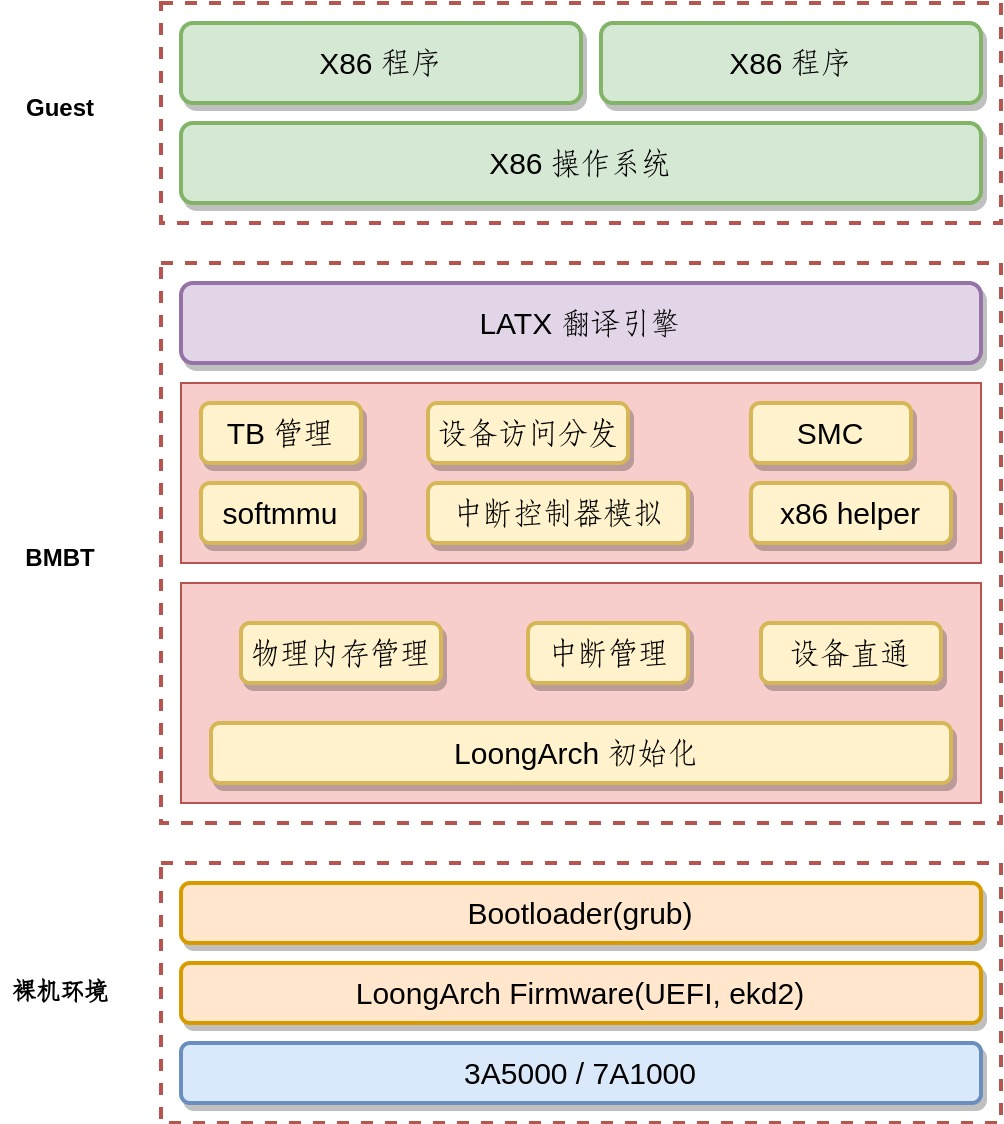
\includegraphics[width=0.8\textwidth]{./images/bmbt.jpg}
	\caption{BMBT 的架构设计}
	\label{fig:bmbt_layout}
\end{figure}

\section{BMBT CPU 虚拟化}
在单位时间内,执行的 Guest 指令的数量越多,二进制翻译器的性能越好,这可以从两个方面来进行优化。
一是,如何让物理 CPU 尽可能多的时间在执行二进制翻译器的代码,而不是会去处理其他任务。二是,如何提升指令的翻译效率。

现代操作系统设计出复杂的调度算法让多个用户进程交替运行,让每一个进程都以为完整地在使用 CPU,但是这导致作为用户进程的二进制翻译器并不是 100\% 占用 CPU 。
在 BMBT 中,首先进行环境的初始化,之后会进入到 Guest 代码的翻译和执行中,一直循环到 Guest 操作系统关机,进而让 Host 关机,
因此可以保证二进制翻译器在翻译执行的过程中,始终是 100\% 占用 CPU 的。
运行在操作系统上的二进制翻译器使用的是一个进程模拟一个 Guest CPU,而 BMBT 是使用一个物理 CPU 来模拟一个物理 CPU,因而消除来操作系统的 CPU 虚拟化的引入开销。

二进制翻译引擎是二进制翻译器的核心,其负责将 Guest 的指令翻译为 Host 的指令。
如图 \ref{fig:tcg} 所示,QEMU 为了尽可能多的支持不同的指令集架构,其开发出来 TCG IR 来作为中间表示层,但是一条 Guest 指令会被翻译为多条 TCG IR 的指令,而一条 TCG IR 指令会进一步翻译为多条 Host 指令,
这导致了高膨胀率,降低了翻译器的执行效率。

\begin{figure}[!htbp]
	\centering
	
\includegraphics[width=1.0\textwidth]{./images/tcg.jpg}
	\caption{TCG}
	\label{fig:tcg}
\end{figure}

而如图 \ref{fig:latx} 所示,LATX 将 TCG 移除掉,采取将 x86 指令直接翻译为 LoongArch 指令的设计,降低了指令膨胀率。

\begin{figure}[!htbp]
	\centering
	
\includegraphics[width=0.6\textwidth]{./images/latx.jpg}
	\caption{LATX}
	\label{fig:latx}
\end{figure}

在 BMBT 中,使用 LoongArch 的 idle 指令来实现 x86 的 halt,因此当 Guest CPU 空闲的时候,可以让物理 CPU 进入低功耗的状态。当 Guest 操作系统的调度器发现无任务调度的时候,会执行 halt 指令,
这是一条特权指令,导致 BMBT 从翻译 TB 执行中退出,并且进入到 halt 指令模拟函数中,之后 BMBT 处理完各种相关工作之后,会打开中断并且执行 idle 指令,进入到低功耗状态。当中断到来的时候,
BMBT 进入到中断处理函数,向 Guest 注入中断,然后执行 idle 的下一条指令,并且从 halt 指令模拟函数中返回,开始翻译执行 halt 的下一条指令,并且在 TB 结束的位置检测到 Guest 中断。

\section{BMBT 设备虚拟化} \label{section:bmbt_device}
和设备驱动相同,设备虚拟化同样需要处理三个方面的问题,\textbf{发送设备命令}和\textbf{设备传输数据}和\textbf{接收设备中断}。

\textbf{设备命令发送},是通过写设备地址空间完成的。PCIe 设备和串口等设备是架构无关的,对于 x86 和 LoongArch 而言,其差别仅仅 PIO和 MMIO 所映射的地址上,
如图 \ref{fig:bmbt_device} 所示,当 Guest 访问设备的时候,只需将访问地址从 x86 的标准调整为 LoongArch 的标准即可。
\begin{figure}[!htbp]
	\centering
	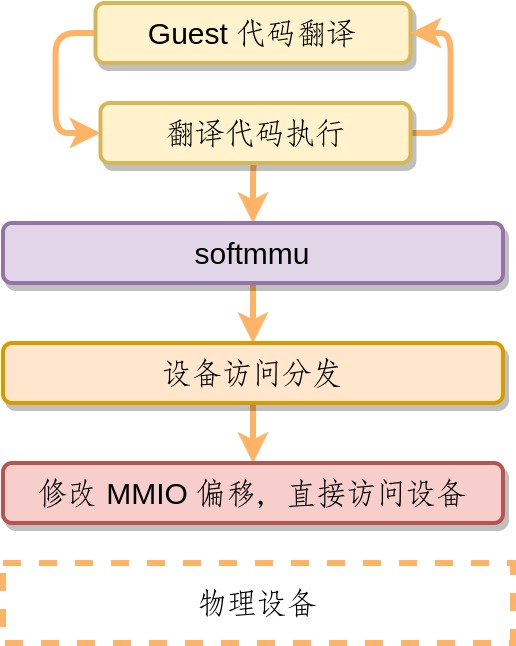
\includegraphics[width=0.6\textwidth]{./images/bmbt-device.jpg}
	\caption{BMBT 的设备虚拟化过程}
	\label{fig:bmbt_device}
\end{figure}

PCI \citep{pci2002express} 是连接外设的高速串行总线标准,PCIe 是 PCI 标准的扩展。
如图 \ref{fig:PCIe} 所示,在 x86 指令集架构中,可以通过 IO 地址为 0xcfc 的 \verb|CONFIG_DATA| 来指定将要访问的 PCI 配置空间的位置,
而通过地址为 0xcf8 的 \verb|CONFIG_CMD| 来提供操作的命令。

在 PCI 配置空间中含有一个 PCIe 设备的基本信息和配置选项。操作系统可以通过设置 Base Address Register (BAR) 和 Expansion ROM Base Address 来将 PCIe MMIO 的操作映射到物理地址空间中。
PCIe 可以通过特殊的 PCI 设备,PCI Bridge,实现层级结构。一个 PCI bridge 的映射窗口决定了挂载在其上所有的 PCI 设备的映射范围。

不同的指令集架构对于 PCI MMIO  的范围有不同的规定,例如 x86 规定范围为 0xe0000000 \textasciitilde 0xfec00000,而 LoongArch 规定为 0x40000000 \textasciitilde 0x80000000,两者没有重叠。
如果只是简单的让 Guest 直接读写 PCI 配置空间,那么在 BAR 中存储的是 x86 的 PCI MMIO 范围的地址,该范围在 LoongArch 是物理内存。
所以在 \ref{fig:PCIe} 的步骤 2 中,如果检测到 Guest 对于 BAR 和 Expansion ROM Base Address 以及 PCI Bridge 映射窗口寄存器进行读写的时候,读写的数值需要做一个大小为 x86 和 LoongArch PCI MMIO 左边界差值的偏移。

\begin{figure}[!htbp]
	\centering
	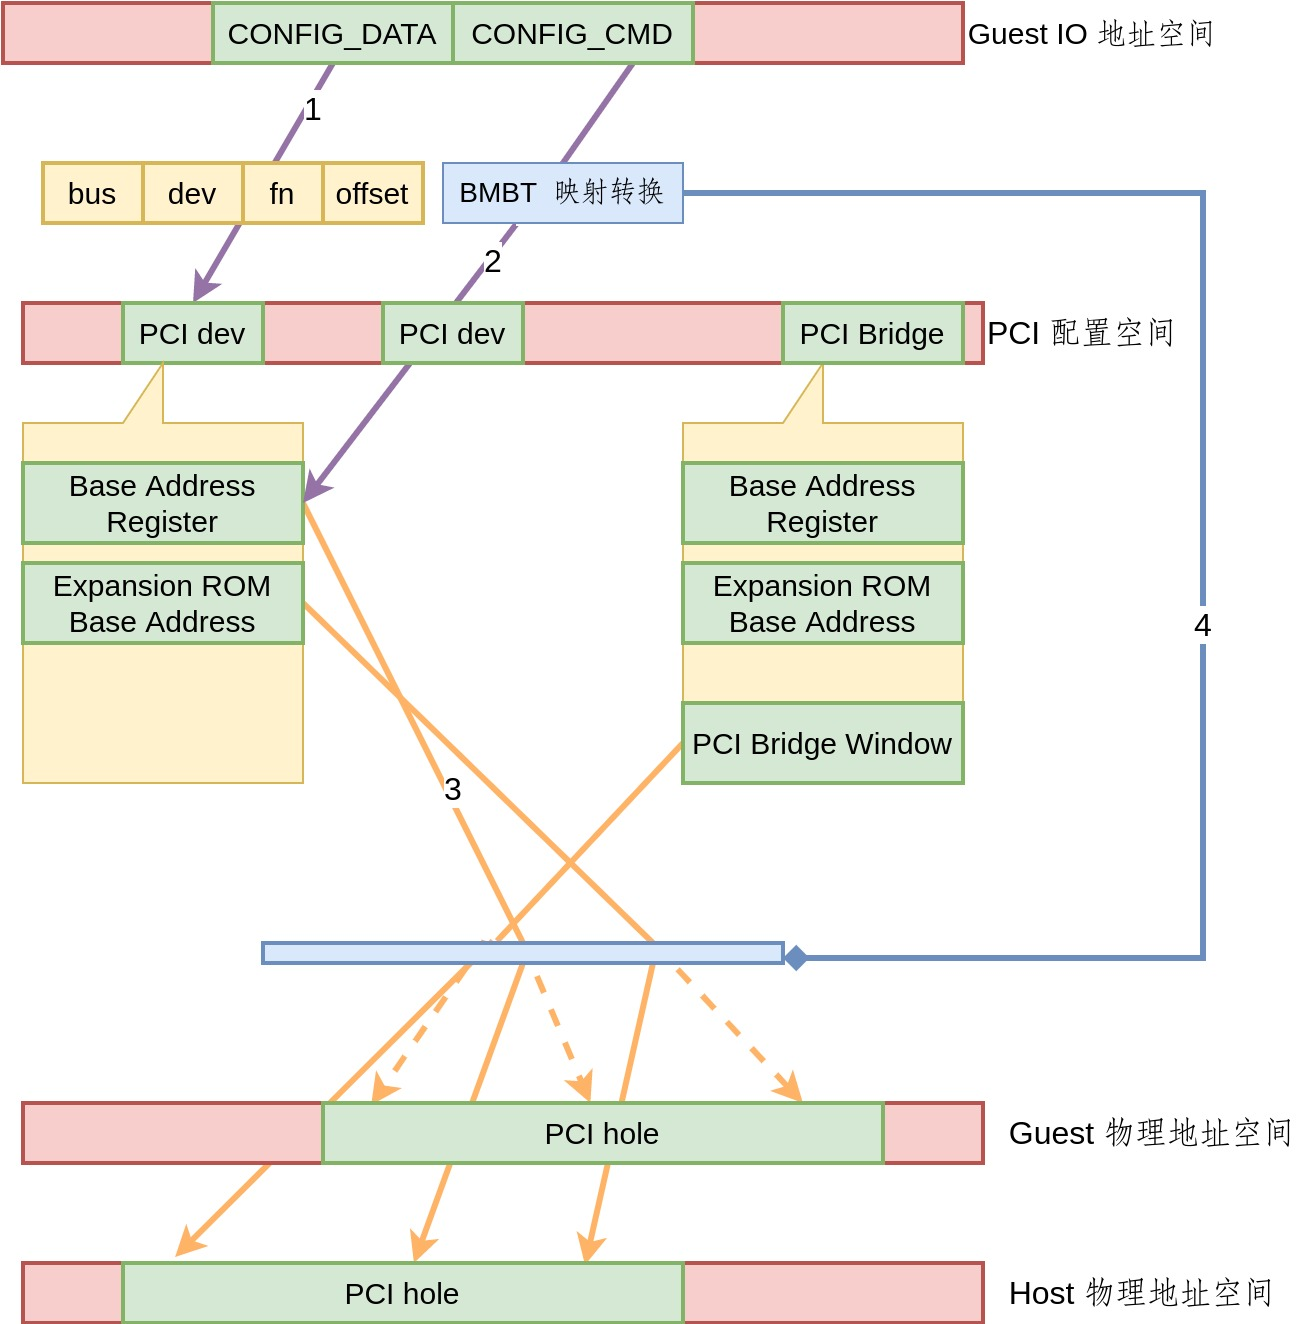
\includegraphics[width=1.0\textwidth]{./images/PCIe.jpg}
	\caption{BMBT 中 PCIe 设备虚拟化的过程}
	\label{fig:PCIe}
\end{figure}

X86 的 bios 启动过程中,需要将 I440FX host PCI bridge 和 PIIX3 PCI to ISA bridge 继续暴露给 Guest 。
i440FX 可以实现 PAM 映射,而 PIIX3 可以用于映射 PCIe Intterrupt Line 的路由。
在 BMBT 中,当访问 I440FX 和 PIIX3 所在的配置空间,将会进行模拟,而不是设备直通。
此外,BMBT 灵活地选择具体暴露出哪一个物理设备给 Guest 使用。

\textbf{设备数据传输} 往往是通过 DMA 完成的,当没有 IOMMU 的时候,并且没有保证 GVA 等于 GPA ,那么会出现图 \ref{fig:bmbt_without_iommu} 中演示问题,
因为 Guest 可以直接访问设备,那么在设备发起 DMA 操作的时候,使用的 GPA 地址为 0x100000,
当设备将数据传写回到物理内存中,其写入的位置实际上是 HPA 的 0x100000 ,
这导致了两个问题,首先,Guest 无法使用 DMA 和 PCIe 沟通,进而导致 PCIe 设备直通失败,其次 Guest 可以操作物理设备访问和破坏 Host 的数据,导致安全问题。
一种简单的解决方法是将让 GPA 等于 HPA,如图 \ref{fig:bmbt_without_iommu2} 所示,但是这还是无法解决安全性问题。

\begin{figure}[!htbp]
	\centering
	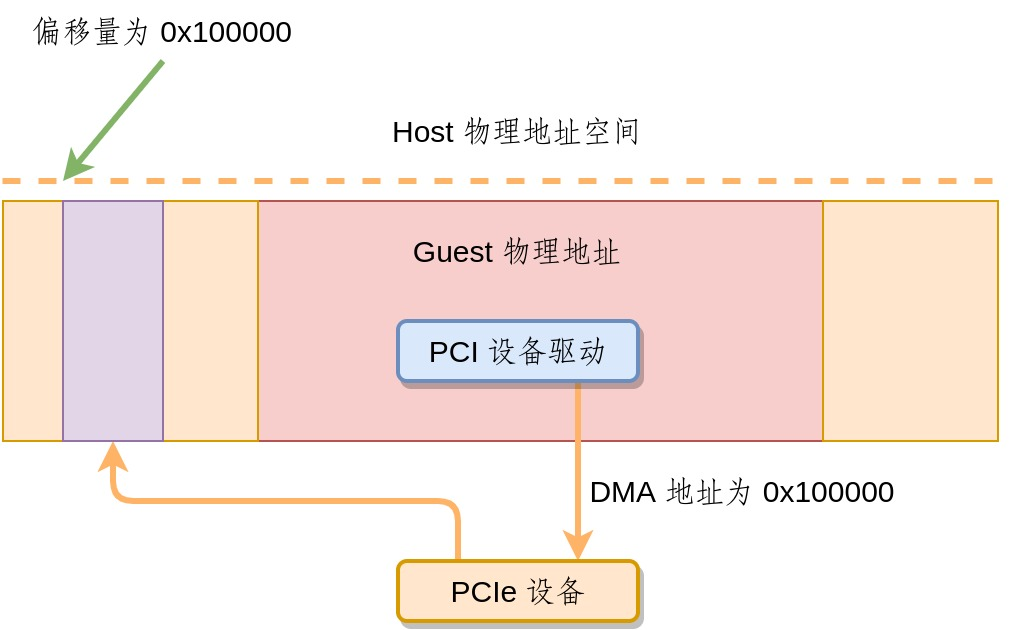
\includegraphics[width=0.8\textwidth]{./images/bmbt-without-iommu.jpg}
	\caption{GPA 不等于 HPA 时候的 DMA 操作}
	\label{fig:bmbt_without_iommu}
\end{figure}

\begin{figure}[!htbp]
	\centering
	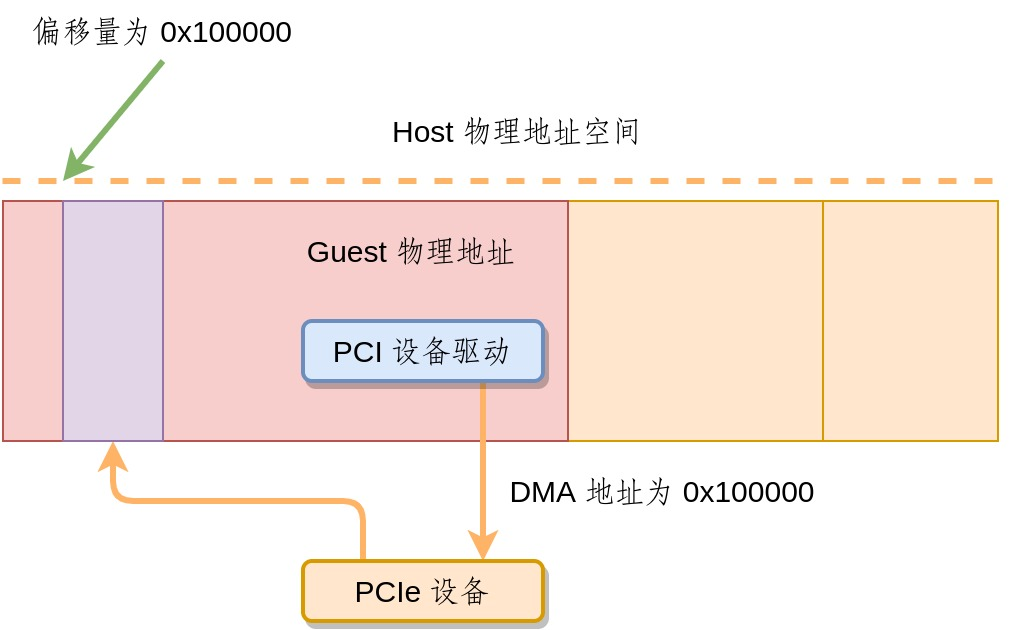
\includegraphics[width=0.8\textwidth]{./images/bmbt-without-iommu2.jpg}
	\caption{GPA 等于 HPA 时候的 DMA 操作}
	\label{fig:bmbt_without_iommu2}
\end{figure}

在未来的工作中,BMBT 会添加上 IOMMU 的支持,从而彻底解决 PCIe 设备 DMA 传输的问题。

\textbf{设备中断接受} 的相关问题在 \ref{section:bmbt:interrupt} 节中讨论。

如果设备直通采用 VFIO 方案,Guest 发送给物理设备的命令需要通过 Linux 内核模块,因此存在用户态系统态上下文切换和内核模块执行的开销。
而 BMBT 只是需要对于设备访问进行偏移的修正,可以将设备模拟的损耗可以忽略不计。

需要注意的是,仅仅和架构无关的设备才可以实现设备直通,如果一个设备是 Guest 独有的,那么只能采用模拟的方法。
考虑只有少数设备是架构相关的,而且在未来设备厂商会尽量避免开发架构独占的设备,以设备直通为主,设备模拟为辅的方案是可行的。
在 BMBT 项目中,主要需要模拟的是 x86 的中断控制器和少数 legacy 设备,例如 mc146818 rtc ,这些设备模拟的实现可以参考 QEMU 。

\section{BMBT 中断虚拟化}\label{section:bmbt:interrupt}
设备可以利用中断主动通知 CPU ,而不是让 CPU 轮询设备的状态。
为了增强中断的灵活性,例如支持多个设备,设置设备中断优先级,屏蔽中断等,设备可以首先将中断发送到
中断控制器,然后中断控制器转发给 CPU 。CPU 可以对于中断控制器进行编程从而来控制中断的发送行为。

现代体系结构为了处理多核,其设计了分层的级联的中断控制器。如图 \ref{fig:x86-intc} 所示是 x86 的中断路由模型,设备首先将中断发送给 IOAPIC 中断控制器,
然后 IOAPIC 中断控制器根据中断路由表将中断转发到目标 Local APIC 上,
最后 Local APIC 将中断发送给其关联的 CPU 上。对于 PCIe 设备,
其中断可以不经过 IOAPIC 转发,通过 MSI 或者 MSI-X 直接中断发送到目标 Local APIC 上。

为了模拟 x86 架构,不仅仅需要可以翻译 x86 指令,同时需要模拟 x86 架构的中断控制器芯片。x86 中断控制器芯片和普通设备的模拟类似,只需要截获对于中断控制器的 IO 操作,然后根据手册模拟其行为即可。

\begin{figure}[!htbp]
	\centering
	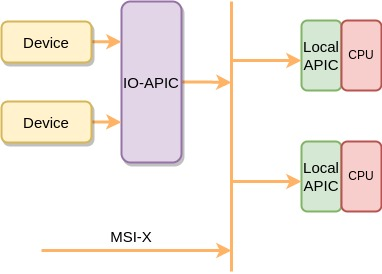
\includegraphics[width=0.5\textwidth]{./images/x86-intc.jpg}
	\caption{x86 中断路由}
	\label{fig:x86-intc}
\end{figure}

\subsection{设备中断模拟}

如果系统级二进制翻译器运行在用户态,例如 QEMU ,那么其需要使用操作系统提供的系统调用来间接地检测模拟设备的中断是否发生。如图 \ref{fig:qemu_interrupt} 所示,
在事件监听线程中调用 epoll 系统调用,进入内核态,如果没有中断到来,操作系统会将事件监听线程设置为阻塞状态,并且去运行其他线程。当中断到来之后,
事件监听线程被操作系统调度器选择,并且从内核态进入到用户态,然后将中断注入到执行线程中。
操作系统需要时钟中断来维持调度器的运行,例如在 Linux 中通常设置 1 秒中接收 1000 次中断,那么意味事件监听线程每秒需要进行 1000 次系统调用和线程切换。
为了最大执行线程的性能,那么事件监听线程不能和执行线程共用 CPU。
p
\begin{figure}[!htbp]
	\centering
	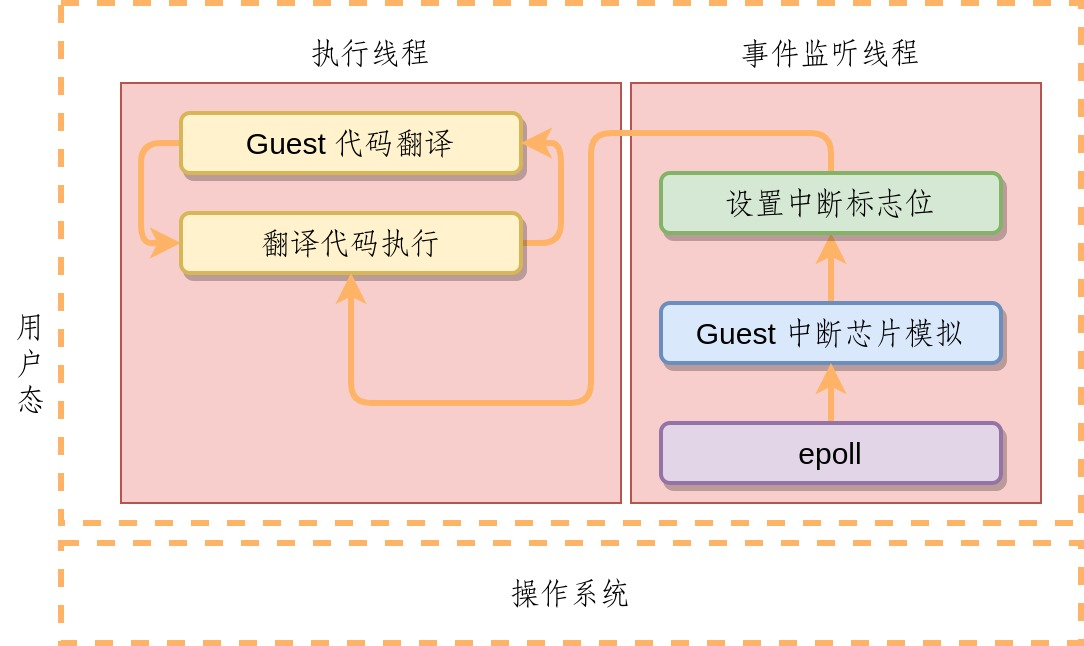
\includegraphics[width=0.8\textwidth]{./images/qemu-interrupt.jpg}
	\caption{QEMU 的中断示意图}
	\label{fig:qemu_interrupt}
\end{figure}

图 \ref{fig:basic_flow4} 展示了动态二进制翻译器的基本运行方式,在其中翻译 TB 会被链接到一起从而避免 Guest 频繁的切换到 Host 中。
对于图 \ref{fig:qemu_interrupt} 这种异步的中断注入模式,如果大量的 TB 被链接到一起或者链接的 TB 中含有循环,那么 Guest CPU 会经过很长时间的延迟才会收到中断。
为了让 Host 接收到中断后,Guest 可以在可接受的延迟内被注入中断,
一种解决方法是在 TB 结束的位置生成两条额外的指令,一条指令检查标志位,一条指令条件跳转。
QEMU 中断的执行流程如图 \ref{fig:qemu_interrupt_flow} 所示。
随着指令翻译效率的提升,这两条指令在翻译 TB 中比例越来越高。

\begin{figure}[!htbp]
	\centering
	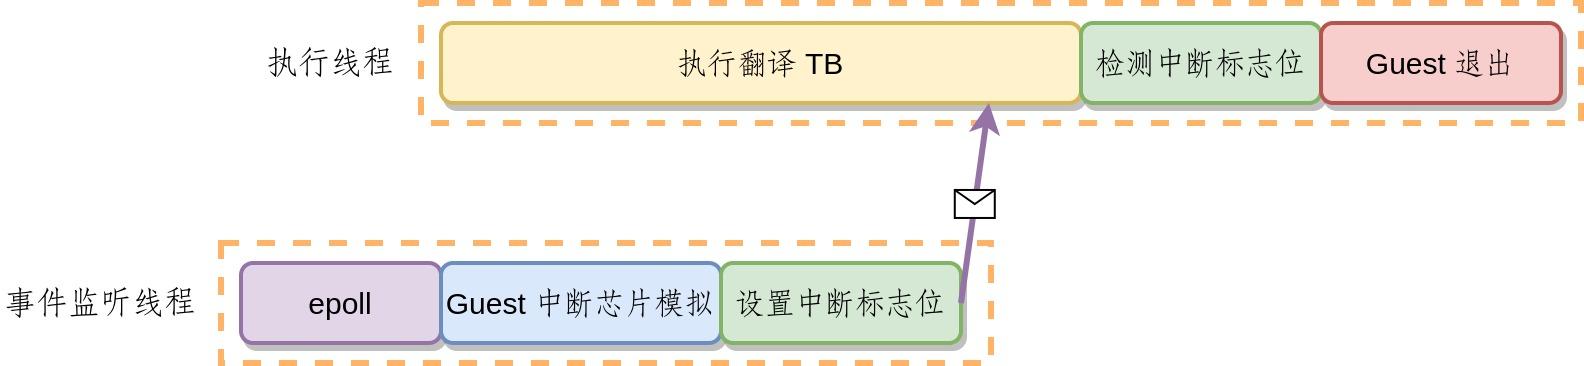
\includegraphics[width=1.0\textwidth]{./images/qemu-interrupt-codeflow.jpg}
	\caption{QEMU 的中断执行流程}
	\label{fig:qemu_interrupt_flow}
\end{figure}

在用户态可以使用信号机制将异步的中断注入转换为同步中断的注入。如图 \ref{fig:signal_interrupt} 所示,生成的翻译 TB 无需额外的中断检查指令,当事件监听线程检测到中断之后,向执行线程发送信号,
执行线程将会跳转到信号处理函数中,在其中可以取消正在执行的 TB 的链接,然后信号处理函数返回。该 TB 执行完成之后,因为其无法知道下一个跳转位置,所以 TB 退出并且检查中断。
虽然这种方案消除每一个生成 TB 的固有的两条中断标志位检测指令,但是需要事件监听线程调用系统调用发送信号,而执行线程只有在中断或者系统调用返回的之后才会开始执行信号处理函数,还是存在一定的延迟。
而且额外的需要多次系统态和用户态的切换。

\begin{figure}[!htbp]
	\centering
	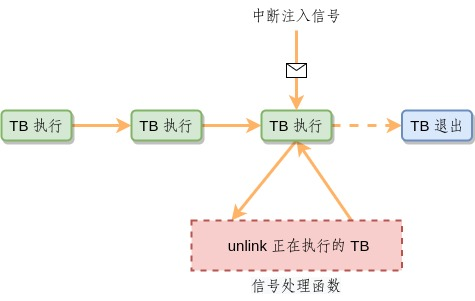
\includegraphics[width=0.7\textwidth]{./images/qemu-signal-interrupt.jpg}
	\caption{基于信号的中断注入}
	\label{fig:signal_interrupt}
\end{figure}

图 \ref{fig:bmbt_interrupt} 是 BMBT 的中断模拟的软件架构,BMBT 无需使用一个额外的线程来进行中断的监听,
当中断到来之后,继续由该 CPU 执行中断的模拟,从而实现每一个物理 CPU 模拟一个 Guest CPU ,无需一个额外的 CPU 来进行事件监听。

\begin{figure}[!htbp]
	\centering
	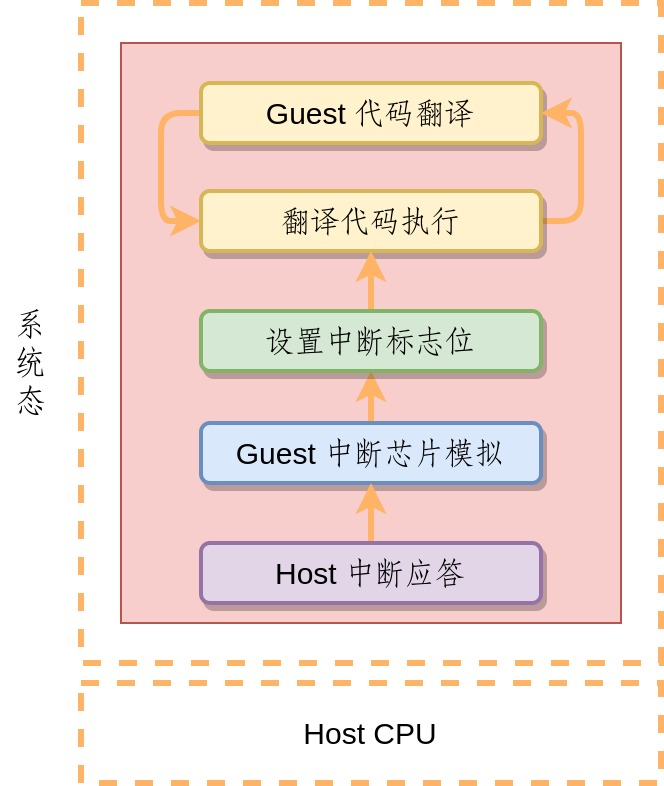
\includegraphics[width=0.5\textwidth]{./images/bmbt-interrupt.jpg}
	\caption{BMBT 的中断软件架构}
	\label{fig:bmbt_interrupt}
\end{figure}

图 \ref{fig:bmbt_interrupt_flow} 展示了在 BMBT 的中断模拟执行流程,
当中断到来之后,CPU 保存上下文,从 TB 执行中切换到 Host 的中断处理函数中,
根据 CPU 和 Host 中断控制器的寄存器的信息确定是哪一个设备发送了中断,也就是 Host 中断应答,
然后调用 Guest 的中断控制器模拟程序来确定发送哪一个中断号给 Guest CPU,
最后设置中断标志位,然后 CPU 会恢复现场,在 TB 结束的位置检测中断标志位并且跳转到 Guest 中断处理函数中。

\begin{figure}[!htbp]
	\centering
	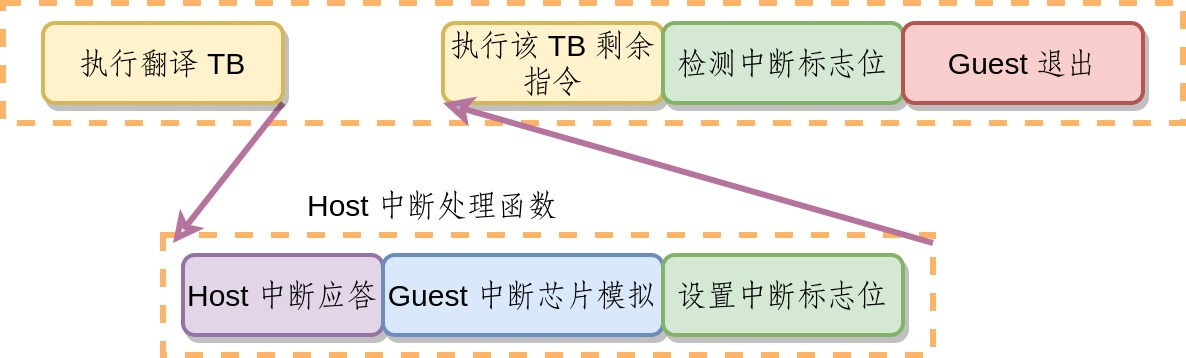
\includegraphics[width=1.0\textwidth]{./images/bmbt-interrupt-codeflow.jpg}
	\caption{BMBT 中的中断流程}
	\label{fig:bmbt_interrupt_flow}
\end{figure}

BMBT 可以消除掉每一个 TB 结束位置的中断标志位检测指令,如图 \ref{fig:bmbt_interrupt_flow2} 所示,在中断处理函数中,
BMBT 可以将正在执行的 TB 从 TB chain 中取出来,因此该 TB 执行完成之后,不会去执行下一个 TB
而会退出到 Host 中,在 Guest 和 Host 中上下文切换中检测中断。

\begin{figure}[!htbp]
	\centering
	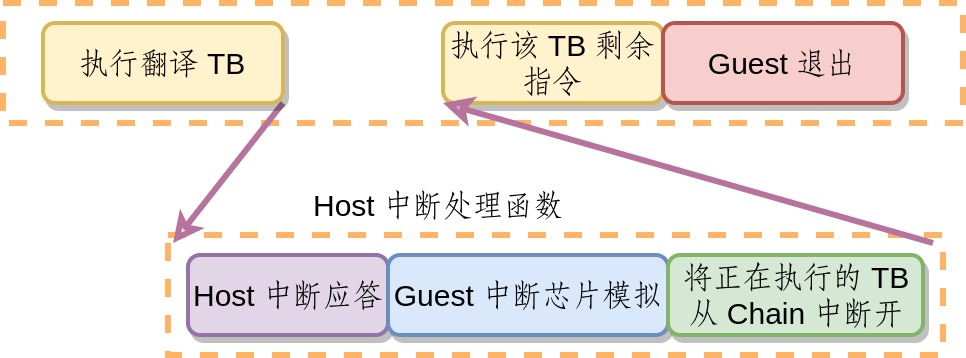
\includegraphics[width=1.0\textwidth]{./images/bmbt-interrupt-codeflow2.jpg}
	\caption{消除中断标志位检测后 BMBT 的执行流程}
	\label{fig:bmbt_interrupt_flow2}
\end{figure}

BMBT 要求 Host 中断控制器的触发模式需要为边沿触发,而不是水平触发。因为在 Host 的中断处理函数中没有应答设备的中断,
如果中断控制器是水平触发,那么退出中断处理函数后会打开中断,接下来中断控制器会继续给 CPU 发送中断,然后开始执行中断处理函数,进而 Host CPU 无法执行其他任务。
即使没有应答设备,边沿触发的中断控制器也只会发送一次中断。考虑到主流的中断控制器默认支持边沿触发或者可以编程其触发模式,这个要求容易满足。

\subsection{时钟中断设计}
x86 Guest 的 rtc ,hpet 和 Local APIC 等设备会发送时钟中断,为了同时模拟多个设备的时钟中断,BMBT 继承了 QEMU 的时钟管理机制,但在其基础上缩减了时钟中断的模拟流程。
如图 \ref{fig:timer_interrupt} 所示,将需要触发的 timer 按照到期时间排序,当 Host CPU 接收到时钟中断的时候,将其中已经到期的所有的 timer 的钩子函数全部执行,
如果其中的钩子函数产生了新的 timer,那么需要插入到 timer 链表中。然后,根据 timer 链表设置最近到期的时钟编程 Host 的计时器下一次触发时钟中断的时间,最后 Host 时钟中断处理函数返回。

\begin{figure}[!htbp]
	\centering
	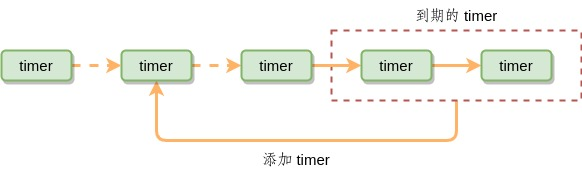
\includegraphics[width=0.9\textwidth]{./images/timer-interrupt.jpg}
	\caption{BMBT 时钟中断模拟}
	\label{fig:timer_interrupt}
\end{figure}

\subsection{MSI 中断设计}
如图 \ref{fig:msi} 所示,是 PCI 配置空间对于 MSI 中断的支持,不同的架构在处理 MSI 中断的时候存在两个不同点,需要进行截获和模拟:
\begin{enumerate}
	\item MSI Address 不同。所以当 Guest 写 PCI hole 空间的时候,首先需要判断是否在写 MSI Address,如果是,那么需要修改为 Host 的 MSI Address。
	\item MSI 分配的中断号的启始位置不同。例如,x86 中从 32 开始分配 MSI 中断号,而 LoongArch 从 64 开始分配中断号,当 Guest 分配从 32 到 63 的中断号会和 Host 其他中断号冲突。
	      所以当 Guest 在写 Data 项的时候,需要进行调整。
\end{enumerate}
\begin{figure}[!htbp]
	\centering
	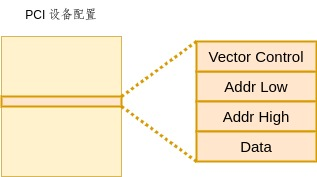
\includegraphics[width=0.5\textwidth]{./images/MSI.jpg}
	\caption{MSI 中断}
	\label{fig:msi}
\end{figure}

\subsection{MSI-X 中断设计}
PCIe 设备可以使用 MSI-X 发送中断,其过程如图 \ref{fig:msix} 所示,PCI 配置空间中的 BAR 确定 MSI-X 表的位置,在 MSI-X 的每一个项中包含 4 个成员。
Addr Low 和 Addr High 一起组成 MSI Address,当 PCIe 设备发送中断的时候会向该地址写第三项数据 Data ,在 Vector Control 中可以屏蔽一个 PCIe 设备的中断。
通过 Data 项,可以控制中断具体发送到哪一个 CPU 的 Local APIC 中。

\begin{figure}[!htbp]
	\centering
	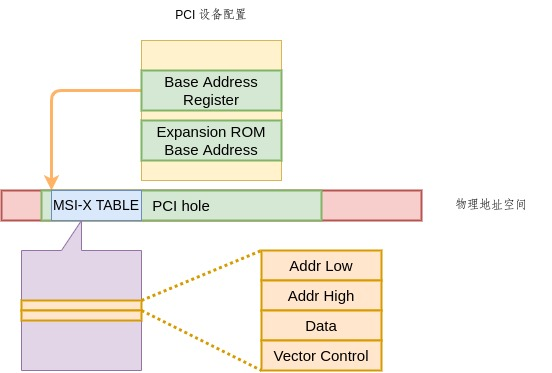
\includegraphics[width=0.8\textwidth]{./images/MSI-X.jpg}
	\caption{MSI-X 中断}
	\label{fig:msix}
\end{figure}

因为 MSI-X 的中断截获发生在 MMIO 中,这意味着 BMBT 需要对于 Guest 的所有的 MMIO 行为进行捕获,判断是否在读写 MSI-X 表。

\section{BMBT 内存虚拟化}
当 bootloader 加载 BMBT 程序之后,BMBT 一直运行在系统态中,不会进入到用户态
因此可以采用 \ref{subsection:memory_virt} 节中提到的使用硬件 TLB 加速 Guest 访存的方案。
相比硬件辅助加速虚拟机,消除 Guest unikernel 导致的虚拟机退出。相对于 Dune,消除了因为用户进程系统调用模拟开销。

如图 \ref{fig:bmbt-layout} 所示,是 BMBT 的物理地址空间。在 \ref{section:bmbt_device} 中指出,因为 BMBT 尚未支持 IOMMU ,需要保持 GPA 等于 HPA ,
所以将 Guest 占用的物理内存从 0 开始,而将其中的空洞来存放 BMBT 的代码段数据段以及 Code Cache,这些物理内存可以通过 e820 或者 ACPI 向 Guest 操作系统隐藏。

\begin{figure}[!htbp]
	\centering
	
\includegraphics[width=1\textwidth]{./images/bmbt-layout.jpg}
	\caption{BMBT 的物理地址空间}
	\label{fig:bmbt-layout}
\end{figure}

LoongArch 架构支持直接映射窗口的功能,可以配置虚拟地址空间和物理地址空间一一映射的范围。
让 BMBT 的访存总是在直接映射窗口上,可以消除 Host 中所有的 TLB 不命中。 如图 \ref{fig:bmbt_gva_hpa} 所示,GVA 到 GPA 的映射可以减少一层,当 Guest TLB 不命中,只需进行 3 次访存。

因为 BMBT 运行在直接映射窗口上,所以 Host 不会占用任何硬件 TLB,当使用硬件 TLB 来加速 Guest 的访存,
在硬件辅助加速虚拟机和 Dune 这两种方案中,Guest 和 Host 都需要使用硬件 TLB,这导致 Guest 和 Host 都无法直接全部的硬件 TLB 来加速各自访存。

\begin{figure}[!htbp]
	\centering
	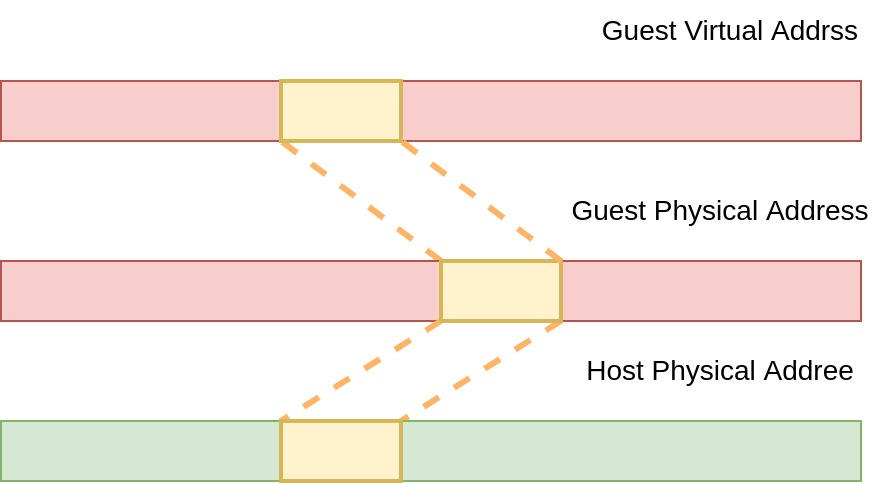
\includegraphics[width=0.7\textwidth]{./images/sys-as3.jpg}
	\caption{BMBT 中 GVA 到 HPA 的映射过程}
	\label{fig:bmbt_gva_hpa}
\end{figure}

\subsection{BMBT 物理页管理}
QEMU 等用户态的二进制翻译器可以调用 Host 操作系统的内存管理系统来分配内存,而 BMBT 直接运行在裸机上,因此需要重新实现高效的一个物理内存管理机制。

现代操作系统,例如 Linux,设计复杂的内存管理机制,其使用 swap 来缓存冷数据,从而节省内存,使用 page cache 来加速存储栈,使用 hugetlb 来提升 TLB 的命中率,
使用 kmemleak 来检测内核内存泄漏,使用 gup 机制来实现内核访问进程的数据,使用 highmem 来处理 32bit 处理器的内存访问等。
之所以 Linux 的物理内存模块非常的复杂,是因为其需要处理各种用户场景。但是 BMBT 需要处理的物理页面分配场景单一,所以可以设计一个更加高效简洁的物理内存分配器。

BMBT 启动之后,通过解析 UEFI 的参数获取物理内存的大小,并且预留 Guest 的物理内存,剩下的内存用于被物理内存分配器管理。
在 BMBT 的运行过程中,分配物理内存的主要原因为:
\begin{enumerate}
	\item 用于实现 Guest 虚拟地址到 TB 的查询的 hashtable 和软件 TLB 会随着运行收缩或扩展。
	\item 管理 TB 从 Host 虚拟地址到 TB 查询的平衡树的大小会随着 TB 数量变化而变化。
	\item LATX 指令翻译的过程中会首先分配内存来存储中间表示等,在翻译完成之后释放。
\end{enumerate}

测试显示,如果简单的采用 Kernighan \& Ritchie malloc (简称 K\&R malloc) 来管理所有的空闲页面,也就是一个链表节点
表示一个空闲物理内存,在运行 SPEC 2000 Test 的过程中会产生超过 100 个链表节点。
但是如果全部采用伙伴系统,伙伴系统只有当分配巧好 $2^n$ 个物理页面的时候才不会浪费物理内存,而且物理页面越大,浪费页面的大小期望越高,
如图 \ref{fig:kr_buddy} 所示,BMBT 混合 K\&R malloc 算法和伙伴算法两种算法,如果分配的物理内存大于 16 个物理页面,那么采用链表,否则采用伙伴系统。采用混合分配算法,在运行 SPEC 2000 的过程中,
K\&R malloc 的链表的节点数始终维持在 5 \textasciitilde 10 之间。在 BMBT 中,大内存的分配的大小较为固定,不容易产生碎片,让小页面的分配使用一个单独的分配器可以防止
大内存和小内存交替分配而产生的碎片。

\begin{figure}[!htbp]
	\centering
	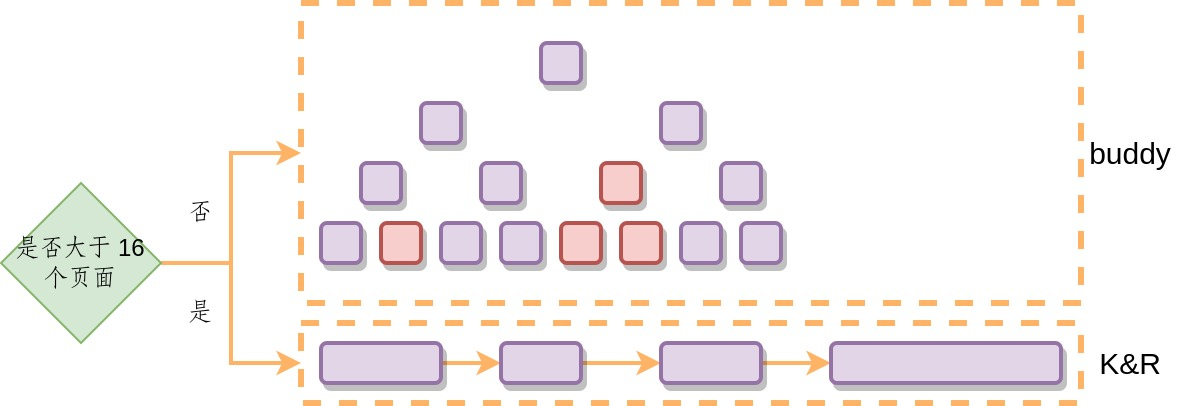
\includegraphics[width=1.0\textwidth]{./images/KR-buddy.jpg}
	\caption{BMBT 的混合内存管理器}
	\label{fig:kr_buddy}
\end{figure}

\section{BMBT 的软件架构}
从零构建一个系统级二进制翻译器在工程上非常有挑战性,MagiXen 就是在 IA-32 EL 进程级二进制翻译器的基础上开发的。
BMBT 主要利用 QEMU 的开发,其软件架构如图 \ref{fig:bmbt_software_arch} 所示,二进制翻译器的主要组成部分为:
\begin{enumerate}
	\item LATX : 高性能的 x86 到 LoongArch 的指令翻译引擎。二进制翻译器的一个难点在于正确性测试,在裸机环境中,调试工具有限,每次更新代码都需要将镜像拷贝到 U 盘中,等待物理机的开机,迭代速度慢。
	      LATX 可以在 QEMU 进行测试,从而减少了开发的难度。
	      而且对于相同的 Guest 程序,在 LATX 和 BMBT 中两者运行的结果相同,可以作为对比调试。
	\item 精简的 QEMU : QEMU 较好的处理了 x86 主板,中断控制芯片和特权指令的模拟,TB 管理,自修改代码,基于 QEMU 开发可以消除这些重复的工作。
	      QEMU 为了模拟各种类型的设备,构建了 QEMU Object Model,为了处理各种架构下的物理内存,其构建了复杂的设备访问分发模型,
	      在 BMBT 中,这些内容可以被精简或者重构。
	\item 精简的 glib : 在 QEMU 依赖于 glib 进行事件监听,内存分配和字符串处理。在 BMBT 中,无需使用 glib 进行事件监听来实现中断,所以 glib 被简化为很薄的 C 库封装层。
	\item 精简的 musl : musl 库相对于 Glibc,其代码结构清晰,便于阅读,BMBT 主要需要利用 musl 提供 malloc ,printf 和浮点库等功能。
\end{enumerate}

\begin{figure}[!htbp]
	\centering
	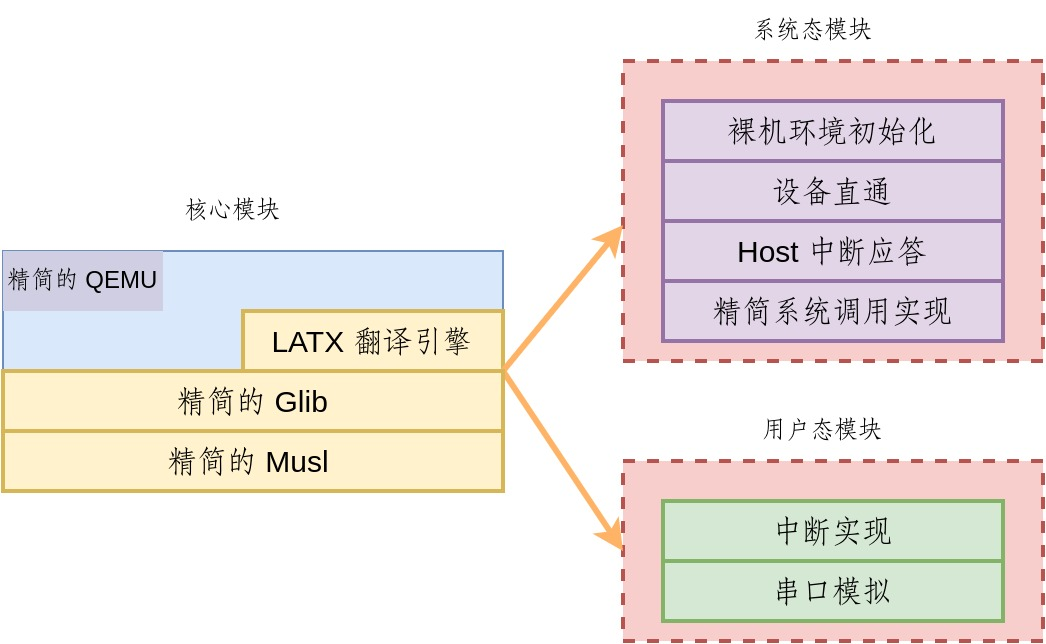
\includegraphics[width=0.9\textwidth]{./images/bmbt-software-arch.jpg}
	\caption{BMBT 软件架构}
	\label{fig:bmbt_software_arch}
\end{figure}

BMBT 可以同时在用户态,KVM 虚拟机和裸机中运行,性能和功能可以逐步增加,但是调试难度也会逐渐增加。
当 BMBT 在 KVM 虚拟机和裸机中运行的时候,使用系统态模块来,主要处理硬件初始化,中断和设备直通。
核心模块中的精简 musl 库需要调用 BMBT 为裸机环境构建的系统调用,主要为 mmap,writev 和 clock\_gettime。

在用户态中,BMBT 只需要支持时钟中断和串口输出,前者是为了维持 Guest 操作系统的进程调度器的运行,而后者是为了调试。
用户态中的时钟中断是通过信号和 posix timer 构建的。

\section{小结}
首先介绍 BMBT 设计思路,并且描述其整体结构。然后本章从 CPU 虚拟化,设备虚拟化,中断虚拟化和内存虚拟化四个角度分析BMBT 的设计。
因为 BMBT 直接运行在裸机上,可以使用物理 CPU 而不是线程来模拟 Guest CPU ,实现设备直通,可以实现同步的中断注入和硬件 TLB 加速访存。
最后,讲解 BMBT 的软件结构以及如何逐步从用户态到虚拟机,最后迭代到裸机上执行。

\chapter{性能分析}\label{chap:result}
本章对于本文提出的 BMBT 进行功能验证和性能测试。
测试的 Host CPU 为 LoongArch 3A5000 ,QEMU 运行的操作系统为基于 Linux kernel 4.19 的 Loongnix 。
测试的 Guest 操作系统为 Linux 内核版本为 4.4.142,其编译选项为 i386\_defconfg,发行版为 Ubuntu Server 32bit 16.04

因为只有 QEMU 支持从 LoongArch 到 x86 的二进制翻译器,所以本文将会使用 QEMU 作为对比,QEMU 的版本为 6.0 。
在 CPU 性能测试中,对比了使用 TCG 作为指令翻译引擎的 QEMU,简称 TCG QEMU, 和使用 LATX 作为指令翻译引擎的 QEMU,简称 LATX QEMU 和 BMBT 的性能。

在 CPU 测试中,使用 SPEC 2000 和 coremark 作为测试基准。
因为设备中断难以直接测试,所以通过硬盘和网络一并测试设备虚拟化和中断虚拟化的效率。
访存上,使用 glibc 的 memcpy 进行测试。
需要注意到,指令翻译引擎性能的提升会同时会加速访存和设备访问,访存的提升同样可以加速 CPU 的执行速度。

\section{CPU 性能测试}

首先使用 coremark 分别对比来 Host ,TCG QEMU,LATX QEMU 和 BMBT 的性能;
\begin{table}[!ht]
	\centering
	\caption{coremark 分数对比}
	\begin{tabular}{|l|l|l|l|l|}
		\hline
		CoreMark & Host  & LATX QEMU & TCG QEMU & BMBT \\ \hline
		score    & 12199 & 2401      & 2031     & 2560 \\ \hline
	\end{tabular}
	\label{table:spec2000_latx_qemu_float}
\end{table}

从 \ref{table:spec2000_latx_qemu_float} 可以看到,因为 LATX 相对于 TCG 存在 21\%
左右的提升,而 BMBT 相对于 LATX QEMU 存在进一步的 6\% 的提升。

\begin{table}[!ht]
	\centering
	\caption{SPEC 2000 定点性能对比}
	\begin{tabular}{|l|l|l|l|}
		\hline
		Testcase      & qemu-latx & bmbt-latx & 加速     \\ \hline
		164.gzip      & 312       & 322       & 03.21\%  \\ \hline
		175.vpr       & 172       & 149       & -13.37\% \\ \hline
		176.gcc       & 319       & 337       & 05.64\%  \\ \hline
		181.mcf       & 1081      & 1313      & 21.46\%  \\ \hline
		186.crafty    & 105       & 167       & 59.05\%  \\ \hline
		197.parser    & 208       & 252       & 21.15\%  \\ \hline
		252.eon       & 91.5      & 100       & 09.29\%  \\ \hline
		253.perlbmk   & 217       & 273       & 25.81\%  \\ \hline
		254.gap       & 144       & 184       & 27.78\%  \\ \hline
		255.vortex    & 204       & 218       & 06.86\%  \\ \hline
		256.bzip2     & 196       & 314       & 60.20\%  \\ \hline
		300.twolf     & 310       & 461       & 48.71\%  \\ \hline
		average score & 222.0     & 268.7     & 21.04 \% \\ \hline
	\end{tabular}
	\label{table:spec2000_latx_qemu_int}
\end{table}

SPEC 2000 定点的平均加速 21\%,其原因来自于多种可能,虽然在执行翻译代码的过程中,BMBT 和 LATX QEMU 的速度相同,
但是在 BMBT 实现了更加高效的物理内存分配器,所以其翻译器运行的更快。并且考虑到 BMBT 消除了所有的 TLB miss ,而且没有用户态和系统态的切换。
其加速程度符合通常的 unikernel 的加速范围。

\begin{table}[!ht]
	\centering
	\caption{SPEC 2000 浮点性能对比}
	\begin{tabular}{|l|l|l|l|}
		\hline
		Testcase      & qemu-latx & bmbt-latx & 加速     \\ \hline
		168.wupwise   & 263.00    & 271.00    & 03.04\%  \\ \hline
		171.swim      & 105.00    & 184.00    & 75.24\%  \\ \hline
		172.mgrid     & 181.00    & 213.00    & 17.68\%  \\ \hline
		173.applu     & 360.00    & 407.00    & 13.06\%  \\ \hline
		177.mesa      & 135.00    & 181.00    & 34.07\%  \\ \hline
		178.galgel    & 776.00    & 788.00    & 01.55\%  \\ \hline
		179.art       & 281.00    & 387.00    & 37.72\%  \\ \hline
		183.equake    & 481.00    & 647.00    & 34.51\%  \\ \hline
		187.facerec   & 600.00    & 598.00    & -0.33\%  \\ \hline
		188.ammp      & 57.20     & 75.60     & 32.17\%  \\ \hline
		189.lucas     & 183.00    & 678.00    & 270.49\% \\ \hline
		191.fma3d     & 214.00    & 222.00    & 03.74\%  \\ \hline
		200.sixtrack  & 253.00    & 207.00    & -18.18\% \\ \hline
		301.apsi      & 143.00    & 393.00    & 174.83\% \\ \hline
		average score & 231.09    & 312.70    & 35.31\%  \\ \hline
	\end{tabular}
	\label{table:spec2000_latx_qemu_fp}
\end{table}
相对定点的 21\% 的提升,在浮点上存在 35.31\% 的提升,一种可能的原因是因为运行在 Host 中,每次上下文切换的时候需要进行浮点寄存器的保存,
而在 BMBT 中运行的时候没有上下文切换,因此也没有浮点寄存器的保存恢复。

\section{IO 性能测试}
使用 dd 和 fio 来测试硬盘设备, 使用 Ping 的延迟来测试网卡。

\begin{table}[!ht]
	\centering
	\caption{dd 硬盘拷贝测试}
	\begin{tabular}{|l|l|l|l|}
		\hline
		Testcase & Host      & LATX QEMU & BMBT         \\ \hline
		dd bs=1G & 292 MB/S  & 31.9 MB/S & 58.5 MB/S \% \\ \hline
		dd bs=4k & 90.9 kB/S & 63.5 kB/s & 77.7 kB/S \% \\ \hline
	\end{tabular}
	\label{fig:dd}
\end{table}

dd 的大块拷贝大约存在 83\% 的提升,而小块拷贝存在 22\% 的提升。
在 BMBT 中,DMA 由硬件完成,而在 QEMU 中,首先硬件将数据拷贝到 Host 的内存中,然后再拷贝到 Guest 内存中,
所以 DMA 操作需要一次额外的拷贝操作。

\begin{table}[!ht]
	\centering
	\caption{LATX QEMU 和 BMBT fio 性能对比}
	\begin{tabular}{|l|l|l|l|}
		\hline
		fio(bs, iodepth, rw) & LATX QEMU (directsync) & BMBT                  & 加速     \\ \hline
		4k, 16, randread     & 5786.2KB/s 10983.36us  & 5371.5KB/s 11731.27us & -7.17\%  \\ \hline
		4k, 16, randwrite    & 1633.9KB/s 39.12ms     & 5417.8KB/s 11728.76us & 231.7\%  \\ \hline
		4k, 1, randread      & 4889.3KB/s 774.74us    & 4686.5KB/s 813.24us   & -4.15\%  \\ \hline
		4k, 1, randwite      & 1393.8KB/s 2.82ms      & 5546.8KB/s 631.78     & 298.13\% \\ \hline
		64m, 4, read         & 302.3MB/s 787.21ms     & 315.3MB/s 765.11ms    & 4.28\%   \\ \hline
		64m, 4, write        & 165.8MB/s 1524.44      & 328.6MB/s 769.82ms    & 98.20\%  \\ \hline
	\end{tabular}
	\label{fig:fio}
\end{table}

使用 fio 在参数 bs iodepth 和 rw 在不同取值的情况下对比性能,bs 描述一次 io 的大小,rw 描述是随机读写还是顺序读写,
iodepth 描述使用 aio 发射队列的大小。从 \ref{fig:fio} 中可以看到,
对于读操作,BMBT 相对于 LATX 没有显著提升,而写操作上,存在平均 189.23\% 的加速。

\begin{table}[!ht]
	\centering
	\caption{含有磁盘 cache 的 LATX QEMU 和 Host 性能比对}
	\begin{tabular}{|l|l|l|}
		\hline
		fio(bs, iodepth, rw) & Host              & LATX QEMU (cache)    \\ \hline
		4k, 16, randread     & 111MB/s 587us     & 8173.5KB/s 7787.98us \\ \hline
		4k, 16, randwrite    & 188MB/s 347us     & 5745.3KB/s 11.09ms   \\ \hline
		4k, 1, randread      & 32.5MB/s 124.35us & 6516.3KB/s 572.93us  \\ \hline
		4k, 1, randwite      & 87.7MB/s 44.94us  & 8325.7KB/s 440.82us  \\ \hline
		64m, 4, read         & 268MB/s 976.55ms  & 353.6MB/s 662.97ms   \\ \hline
		64m, 4, write        & 343MB/s 770.65ms  & 495.4MB/s 507.14ms   \\ \hline
	\end{tabular}
	\label{fig:fio_nocache}
\end{table}

不过需要注意的是,在 QEMU 中进行 fio 的测试的时候,设备是否使用 Host 的 page cache 存在相当大的影响,在表 \ref{fig:fio_nocache} 中对比了
Host 和使用 page cache 的 LATX QEMU 的 fio 性能,在 (bs,iodepth,write)=(64m, 4, write) 的测试中,LATX QEMU 的性能可以比 Host 更高。

分别在 Host ,QEMU 和 BMBT 中 Ping 局域网中相同的一台电脑的延迟如图 \ref{fig:Ping} 所示,
在 BMBT 和 Host 中 Ping 的延迟更低,而且延迟的变化更小,因为在 QEMU 网卡的模拟是在 IO 线程进行的,
Ping 发送请求之后就会进入到等待状态,所以 Ping 延迟取决于会被 IO 线程的执行速度。而在 BMBT 中直接访问物理网卡,无需模拟。

\begin{figure}[!htbp]
	\centering
	\includegraphics[width=0.8\textwidth]{./images/Ping.png}
	\caption{Ping 延迟测试}
	\label{fig:Ping}
\end{figure}

\section{访存性能测试}
使用 glibc 的 memcpy 进行访存测试,首先 mmap 两个大小为 100M 的虚拟地址空间,然后调用 memcpy 多次拷贝,取平均数值。

\begin{table}[!ht]
	\centering
	\caption{glibc memcpy 测试}
	\begin{tabular}{|l|l|l|l|l|}
		\hline
		Host          & LATX QEMU     & BMBT          & 加速    \\ \hline
		8.555453 GB/s & 0.016563 GB/s & 0.021312 GB/s & 28.67\% \\ \hline
	\end{tabular}
	\label{fig:glibc_memcpy}
\end{table}
memcpy 加速 28.67\%,其主要来源让 GVA 到 HPA 的映射从 4 层映射修改为 3 层,从而消除所有的 TLB miss。

\section{小结}
从 CPU IO 和访存三个方面进行测试,发现 BMBT 在 SPEC 2000 定点上存在 21\% 的提升,SPEC 2000 浮点存在 35\% 。
在 fio 的读写测试中,虽然在读操作上不存在显著差异,但是在写操作有 189.23\% 的提升。
在访存上测试,memcpy 有 28.67\% 的提升。

BMBT 已经取得了不错的性能提升,但是更加重要的是,因为 BMBT 运行在系统态中,为进一步的优化提供了空间。

\chapter{总结和展望}\label{chap:future}

\section{总结}
本文分析系统级二进制翻译的挑战,并且提出了通用且有效的方案,BMBT,来解决其中最为关键的挑战,也就是如何提升跨架构二进制翻译器的性能。
相比与 Transmeta Code Morphing 或者 IBM Daisy,BMBT 无需额外的特殊的硬件支持。LoongArch 不是超标量架构,
所以 BMBT 可以较为容易的迁移到 MIPS,ARM,RISC-V 等其他主流的指令集架构上。
同时 BMBT 不是运行在虚拟机或者用户态,而是直接运行在系统态,这消除了 Host 操作系统的软件栈,并且让二进制翻译器可以直接访问硬件资源,从而提升二进制翻译器的性能。

实验结果表明,对于同样使用 LATX 翻译引擎的 QEMU 相比,在 SPEC 2000 定点和浮点测试上,BMBT 分别存在 21\% 和 35\% 的提升。
在 fio 的写测试中,BMBT 取得了 189.23\% 的提升。
memcpy 测试显示 BMBT 有 28.67\% 性能提升。

\section{展望}
跨架构系统级二进制翻译器是消除指令集架构的关键方法,运行在用户态的二进制翻译器难以或者无法高效实现的优化可以轻松地在系统态中实现,
裸金属二进制翻译器的提出为系统级二进制翻译提出了一个新的创新平台,在其基础上可以进行一系列的优化。

\subsection{进一步的优化}
\begin{enumerate}
	\item CPU 虚拟化。当前 BMBT 只能让一个 Host CPU 模拟一个 Guest CPU ,其他的物理 CPU 处于休眠的状态。
	      QEMU 可以使用多线程模拟多个物理 CPU\citep{cota2017cross},在未来的工作中,BMBT 可以将所有的物理 CPU 利用上,从而支持一个多核 Guest 的运行。
	      此外,LATX 的翻译是基于 TB 的,翻译函数是基于每一条指令构建的,没有利用整个函数的信息进行优化,导致生成的指令质量不高。
	\item 中断虚拟化。为了让 Guest 可以及时的检测是否存在中断的注入,需要在每一个 TB 结束的位置额外增加两条指令来检测中断标志位。
	      在 BMBT 中可以采用图\ref{fig:bmbt_interrupt_flow2} 所示的方案,当接收到中断之后,
	      可以取消正在执行的 TB 的链接,因此中断检测指令放到 Guest 和 Host 的上下文切换中。
	\item 设备虚拟化。虽然支持设备直通可以消除设备的模拟,但是因为 Host 和 Guest 的物理地址空间中,设备 IO 地址空间的范围不同,所以需要进行转换,
		可以利用 IOMMU 和 TLB 来压缩从 Guest 的设备访问指令的开销。
	\item 内存虚拟化。 BMBT 尚未实现硬件 TLB 加速 Guest 访存,这导致 Guest 的每条 x86 访存指令至少需要 11 条额外的 LoongArch 指令模拟软件 TLB 。
		在未来的工作中可以实现图 \ref{fig:hamt} 所示的硬件 TLB 加速 Guest 访存。
\end{enumerate}

提出 BMBT 的一个主要目的是为了验证在裸金属上运行二进制翻译器的可行性,虽然 BMBT 在工程实现上使用多种技巧减少工作量,加速项目的推进,但是现有工作的还有一些完善的地方。
\subsection{现有工作的完善}
\begin{enumerate}
	\item 集成性能分析工具。利用上硬件性能计数器可以精确的分析代码的热点,定位性能瓶颈,硬件性能计数器的驱动可以在未来的工作中添加上。
	\item 支持 amd64 的架构。在 BMBT 开发的过程中,LATX 指令翻译器引擎尚且不支持 从 LoongArch 到 amd64 的翻译,所以 BMBT 暂时没有考虑 amd64 架构支持。
	\item 支持 Windows 操作系统。因为 Linux 操作系统是开源的,将 Linux 作为 Guest 可以通过分析源代码来辅助调试,BMBT 在执行路径上要求默认是 Linux,在未来的工作中可以增强 BMBT 的兼容性,
		从而支持任意的操作系统。
	\item 支持 ACPI。因为没有支持 ACPI,导致 PCIe 的 ECAM 空间,物理 CPU 的数量等硬件信息需要被硬编码,这减低了 BMBT 的可移植性。
	\item 支持 UEFI 固件。UFIE 固件加载了 bootloader 之后,其所占用的物理内存会被 Guest 使用,因而后续无法使用 UEFI 的功能。
	\item 利用 IOMMU 实现设备直通。在没有 IOMMU 的支持的情况下实现设备直通,需要保证要求 GPA 等于 HVA,而且 Guest 可以控制物理设备直接读写任意位置位置的物理内存,这既降低了灵活性,也带来了安全性问题。
\end{enumerate}
